% Options for packages loaded elsewhere
\PassOptionsToPackage{unicode}{hyperref}
\PassOptionsToPackage{hyphens}{url}
\PassOptionsToPackage{dvipsnames,svgnames,x11names}{xcolor}
%
\documentclass[
  letterpaper,
  DIV=11,
  numbers=noendperiod,
  titlepage]{scrartcl}

\usepackage{amsmath,amssymb}
\usepackage{iftex}
\ifPDFTeX
  \usepackage[T1]{fontenc}
  \usepackage[utf8]{inputenc}
  \usepackage{textcomp} % provide euro and other symbols
\else % if luatex or xetex
  \usepackage{unicode-math}
  \defaultfontfeatures{Scale=MatchLowercase}
  \defaultfontfeatures[\rmfamily]{Ligatures=TeX,Scale=1}
\fi
\usepackage{lmodern}
\ifPDFTeX\else  
    % xetex/luatex font selection
\fi
% Use upquote if available, for straight quotes in verbatim environments
\IfFileExists{upquote.sty}{\usepackage{upquote}}{}
\IfFileExists{microtype.sty}{% use microtype if available
  \usepackage[]{microtype}
  \UseMicrotypeSet[protrusion]{basicmath} % disable protrusion for tt fonts
}{}
\makeatletter
\@ifundefined{KOMAClassName}{% if non-KOMA class
  \IfFileExists{parskip.sty}{%
    \usepackage{parskip}
  }{% else
    \setlength{\parindent}{0pt}
    \setlength{\parskip}{6pt plus 2pt minus 1pt}}
}{% if KOMA class
  \KOMAoptions{parskip=half}}
\makeatother
\usepackage{xcolor}
\usepackage[top=20mm,bottom=5mm]{geometry}
\setlength{\emergencystretch}{3em} % prevent overfull lines
\setcounter{secnumdepth}{-\maxdimen} % remove section numbering
% Make \paragraph and \subparagraph free-standing
\ifx\paragraph\undefined\else
  \let\oldparagraph\paragraph
  \renewcommand{\paragraph}[1]{\oldparagraph{#1}\mbox{}}
\fi
\ifx\subparagraph\undefined\else
  \let\oldsubparagraph\subparagraph
  \renewcommand{\subparagraph}[1]{\oldsubparagraph{#1}\mbox{}}
\fi


\providecommand{\tightlist}{%
  \setlength{\itemsep}{0pt}\setlength{\parskip}{0pt}}\usepackage{longtable,booktabs,array}
\usepackage{calc} % for calculating minipage widths
% Correct order of tables after \paragraph or \subparagraph
\usepackage{etoolbox}
\makeatletter
\patchcmd\longtable{\par}{\if@noskipsec\mbox{}\fi\par}{}{}
\makeatother
% Allow footnotes in longtable head/foot
\IfFileExists{footnotehyper.sty}{\usepackage{footnotehyper}}{\usepackage{footnote}}
\makesavenoteenv{longtable}
\usepackage{graphicx}
\makeatletter
\def\maxwidth{\ifdim\Gin@nat@width>\linewidth\linewidth\else\Gin@nat@width\fi}
\def\maxheight{\ifdim\Gin@nat@height>\textheight\textheight\else\Gin@nat@height\fi}
\makeatother
% Scale images if necessary, so that they will not overflow the page
% margins by default, and it is still possible to overwrite the defaults
% using explicit options in \includegraphics[width, height, ...]{}
\setkeys{Gin}{width=\maxwidth,height=\maxheight,keepaspectratio}
% Set default figure placement to htbp
\makeatletter
\def\fps@figure{htbp}
\makeatother

\usepackage{booktabs}
\usepackage{longtable}
\usepackage{array}
\usepackage{multirow}
\usepackage{wrapfig}
\usepackage{float}
\usepackage{colortbl}
\usepackage{pdflscape}
\usepackage{tabu}
\usepackage{threeparttable}
\usepackage{threeparttablex}
\usepackage[normalem]{ulem}
\usepackage{makecell}
\usepackage{xcolor}
\usepackage{typearea}
\KOMAoption{captions}{tableheading}
\makeatletter
\makeatother
\makeatletter
\makeatother
\makeatletter
\@ifpackageloaded{caption}{}{\usepackage{caption}}
\AtBeginDocument{%
\ifdefined\contentsname
  \renewcommand*\contentsname{Table of contents}
\else
  \newcommand\contentsname{Table of contents}
\fi
\ifdefined\listfigurename
  \renewcommand*\listfigurename{List of Figures}
\else
  \newcommand\listfigurename{List of Figures}
\fi
\ifdefined\listtablename
  \renewcommand*\listtablename{List of Tables}
\else
  \newcommand\listtablename{List of Tables}
\fi
\ifdefined\figurename
  \renewcommand*\figurename{Figure}
\else
  \newcommand\figurename{Figure}
\fi
\ifdefined\tablename
  \renewcommand*\tablename{Table}
\else
  \newcommand\tablename{Table}
\fi
}
\@ifpackageloaded{float}{}{\usepackage{float}}
\floatstyle{ruled}
\@ifundefined{c@chapter}{\newfloat{codelisting}{h}{lop}}{\newfloat{codelisting}{h}{lop}[chapter]}
\floatname{codelisting}{Listing}
\newcommand*\listoflistings{\listof{codelisting}{List of Listings}}
\makeatother
\makeatletter
\@ifpackageloaded{caption}{}{\usepackage{caption}}
\@ifpackageloaded{subcaption}{}{\usepackage{subcaption}}
\makeatother
\makeatletter
\@ifpackageloaded{tcolorbox}{}{\usepackage[skins,breakable]{tcolorbox}}
\makeatother
\makeatletter
\@ifundefined{shadecolor}{\definecolor{shadecolor}{rgb}{.97, .97, .97}}
\makeatother
\makeatletter
\makeatother
\makeatletter
\makeatother
\ifLuaTeX
  \usepackage{selnolig}  % disable illegal ligatures
\fi
\IfFileExists{bookmark.sty}{\usepackage{bookmark}}{\usepackage{hyperref}}
\IfFileExists{xurl.sty}{\usepackage{xurl}}{} % add URL line breaks if available
\urlstyle{same} % disable monospaced font for URLs
\hypersetup{
  pdftitle={Simulation Result For Two-Level Slope Model With High Prevalence},
  pdfauthor={Shafayet Khan Shafee},
  colorlinks=true,
  linkcolor={blue},
  filecolor={Maroon},
  citecolor={Blue},
  urlcolor={Blue},
  pdfcreator={LaTeX via pandoc}}

\title{Simulation Result For Two-Level Slope Model With High Prevalence}
\usepackage{etoolbox}
\makeatletter
\providecommand{\subtitle}[1]
\author{Shafayet Khan Shafee}
\date{25 August 2023}

\begin{document}
\maketitle
\ifdefined\Shaded\renewenvironment{Shaded}{\begin{tcolorbox}[sharp corners, breakable, frame hidden, enhanced, boxrule=0pt, interior hidden, borderline west={3pt}{0pt}{shadecolor}]}{\end{tcolorbox}}\fi

\newpage

\hypertarget{histograms-for-logwidehatmor-when-number-of-cluster-is-10}{%
\section{\texorpdfstring{Histograms for \(log(\widehat{MOR})\) When
Number of Cluster is
10}{Histograms for log(\textbackslash widehat\{MOR\}) When Number of Cluster is 10}}\label{histograms-for-logwidehatmor-when-number-of-cluster-is-10}}

\vspace{5mm}

\begin{figure}

\begin{minipage}[t]{0.50\linewidth}

{\centering 

\raisebox{-\height}{

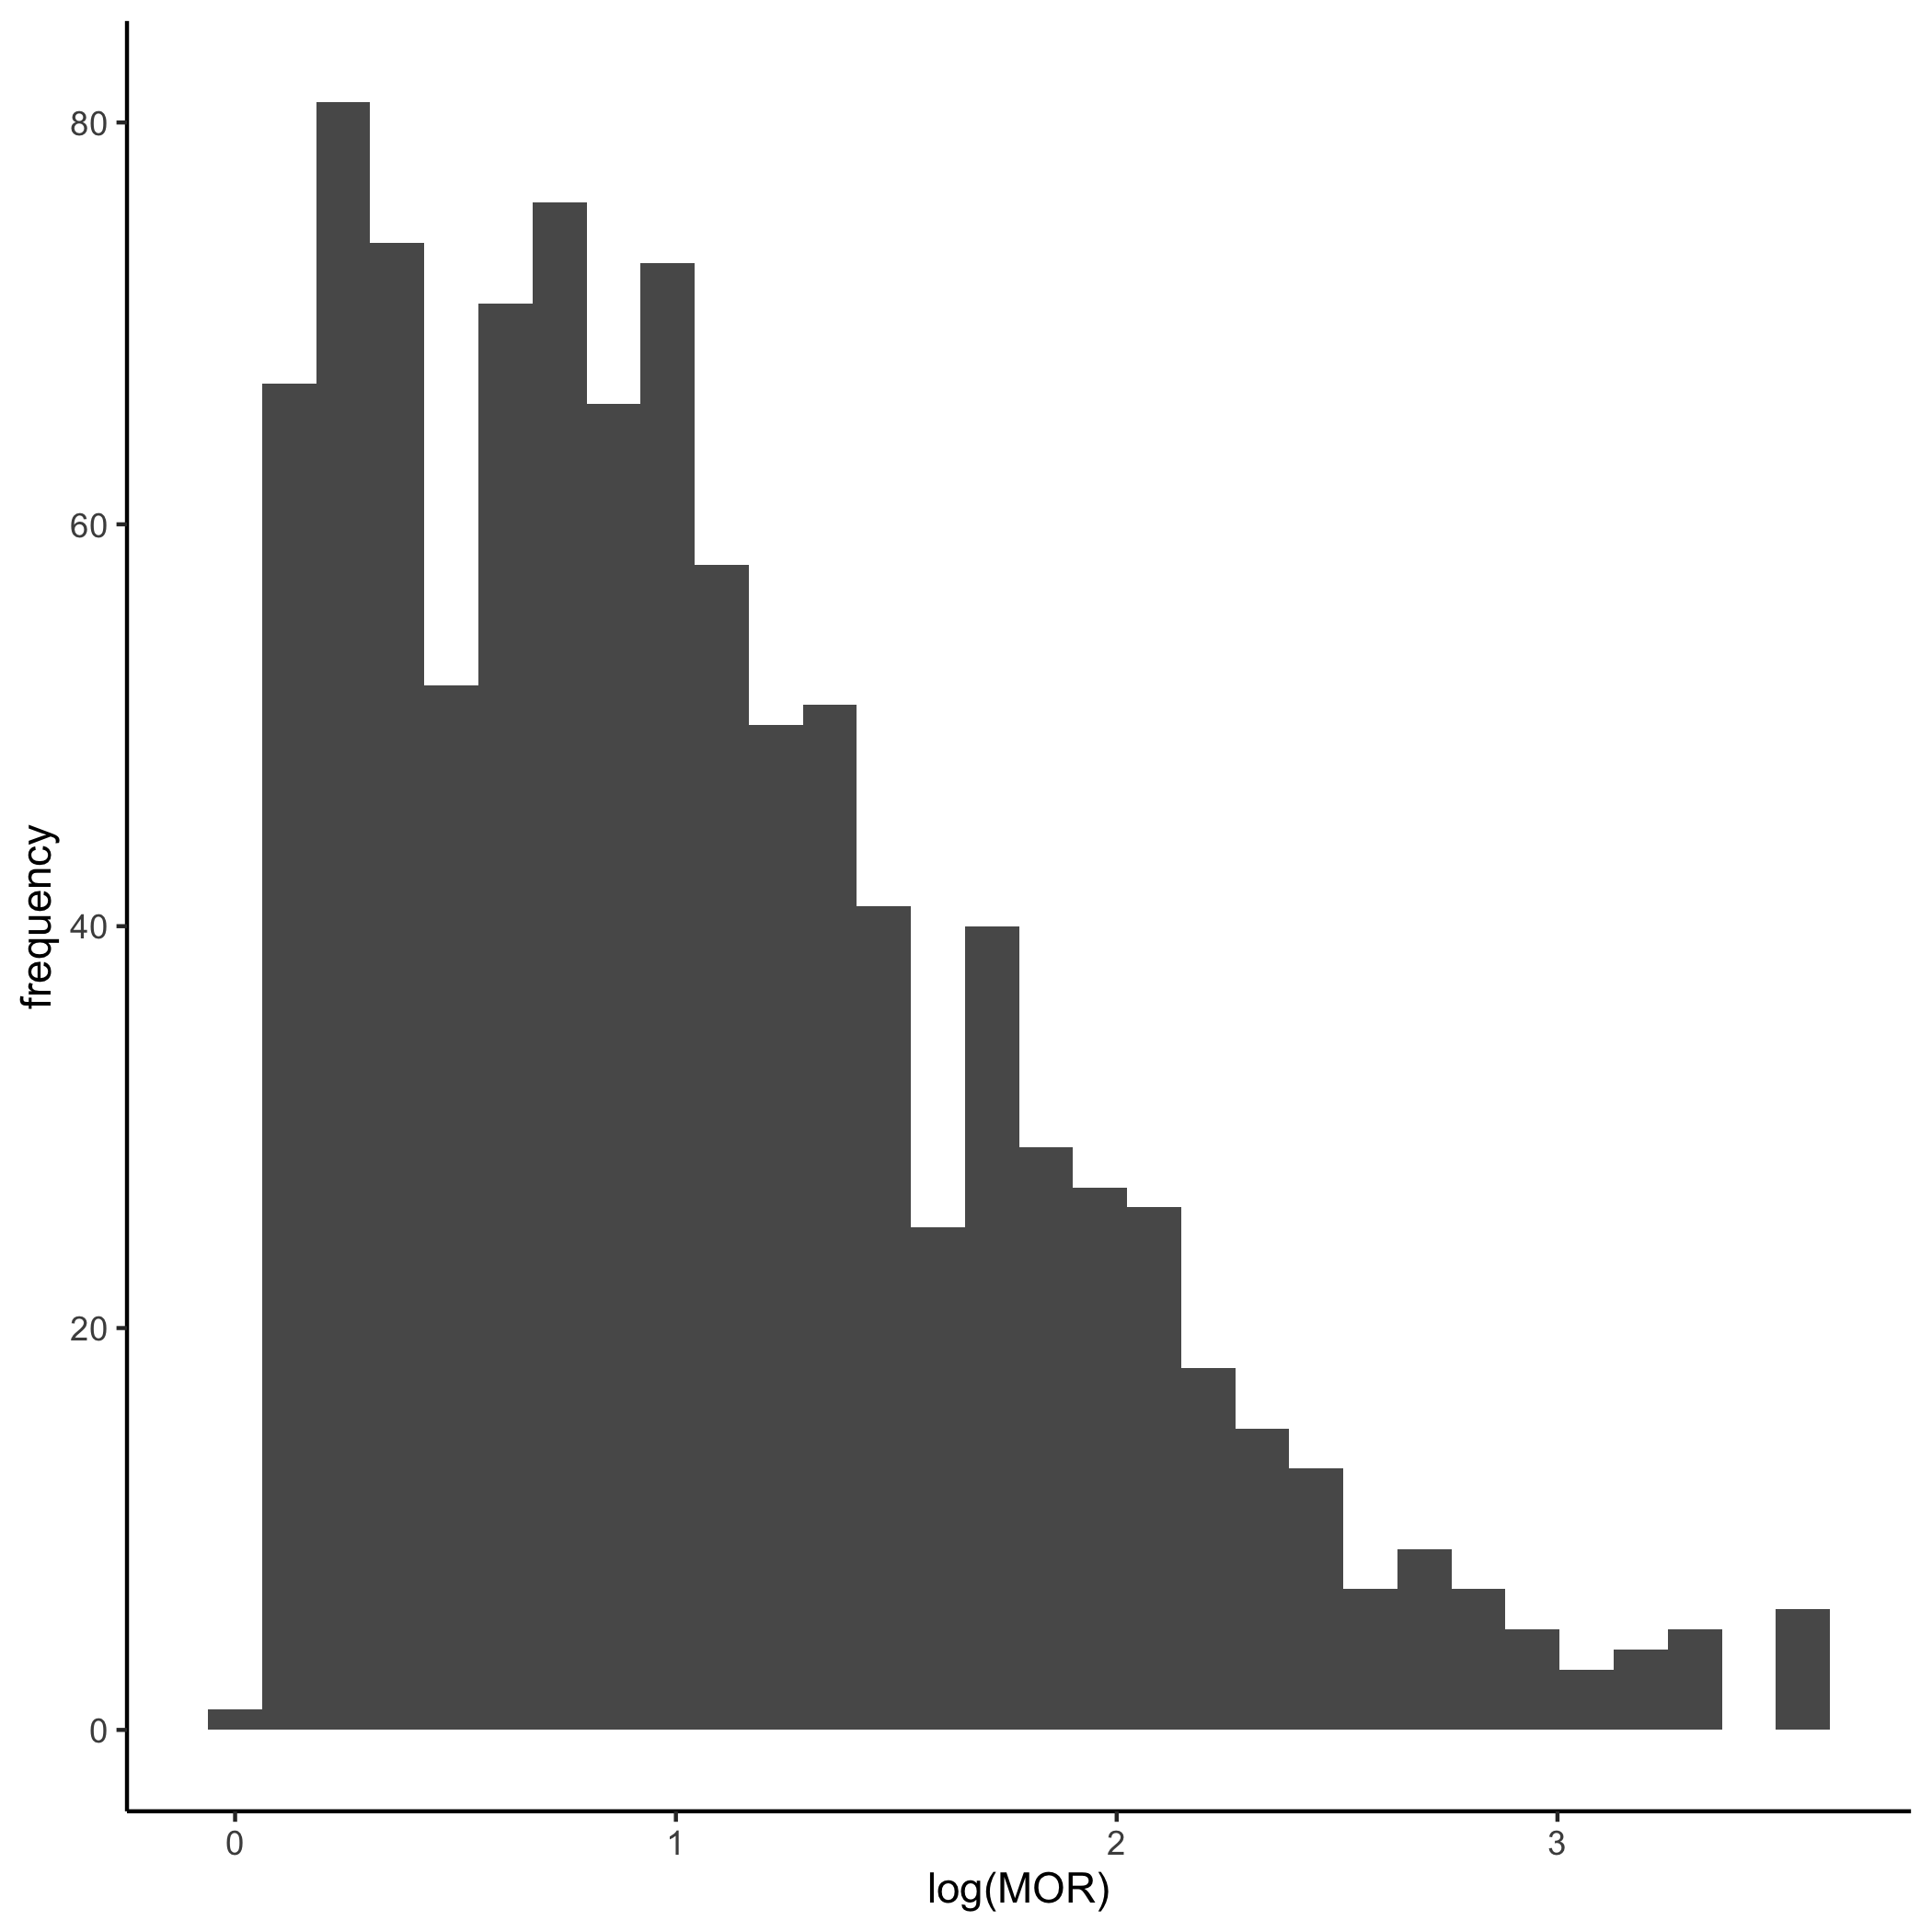
\includegraphics{../../plots/two-lvl-ran-slope/high-prev/hist_10_5_two_lvl_slp_high_prev.png}

}

\caption{For cluster size 5}

}

\end{minipage}%
%
\begin{minipage}[t]{0.50\linewidth}

{\centering 

\raisebox{-\height}{

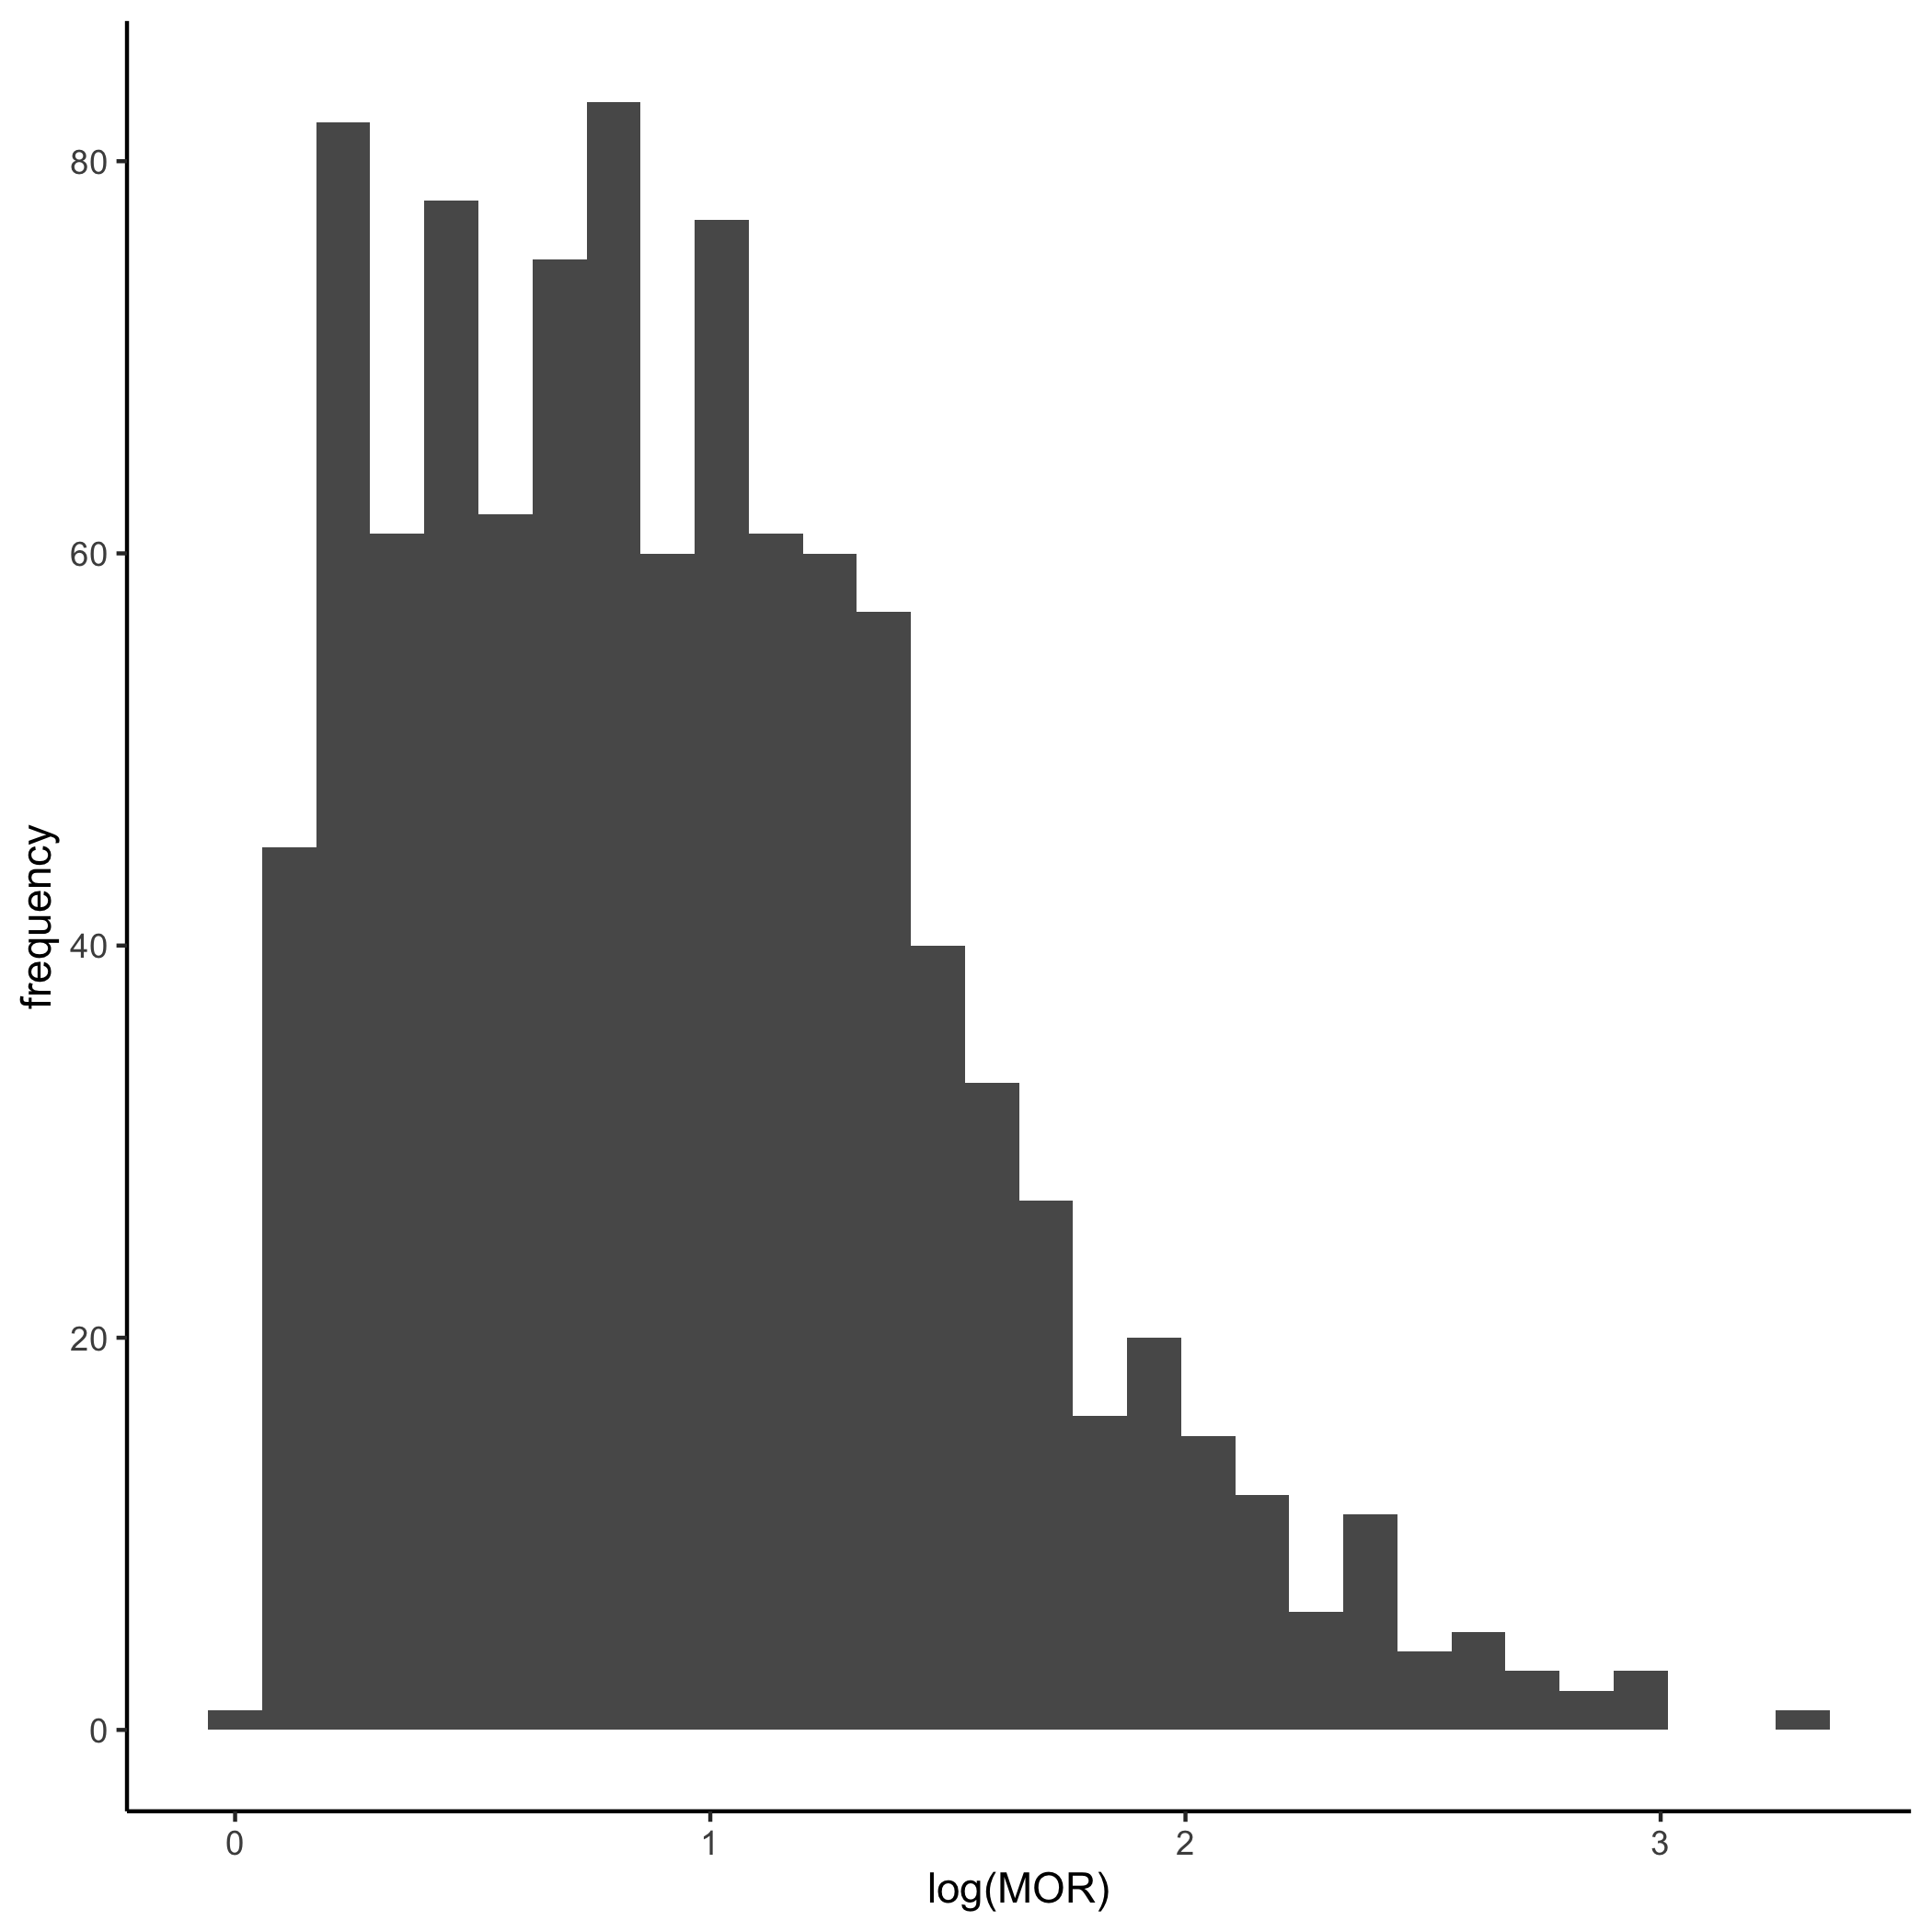
\includegraphics{../../plots/two-lvl-ran-slope/high-prev/hist_10_10_two_lvl_slp_high_prev.png}

}

\caption{For cluster size 10}

}

\end{minipage}%
\newline
\begin{minipage}[t]{\linewidth}

{\centering 

~

}

\end{minipage}%
\newline
\begin{minipage}[t]{0.50\linewidth}

{\centering 

\raisebox{-\height}{

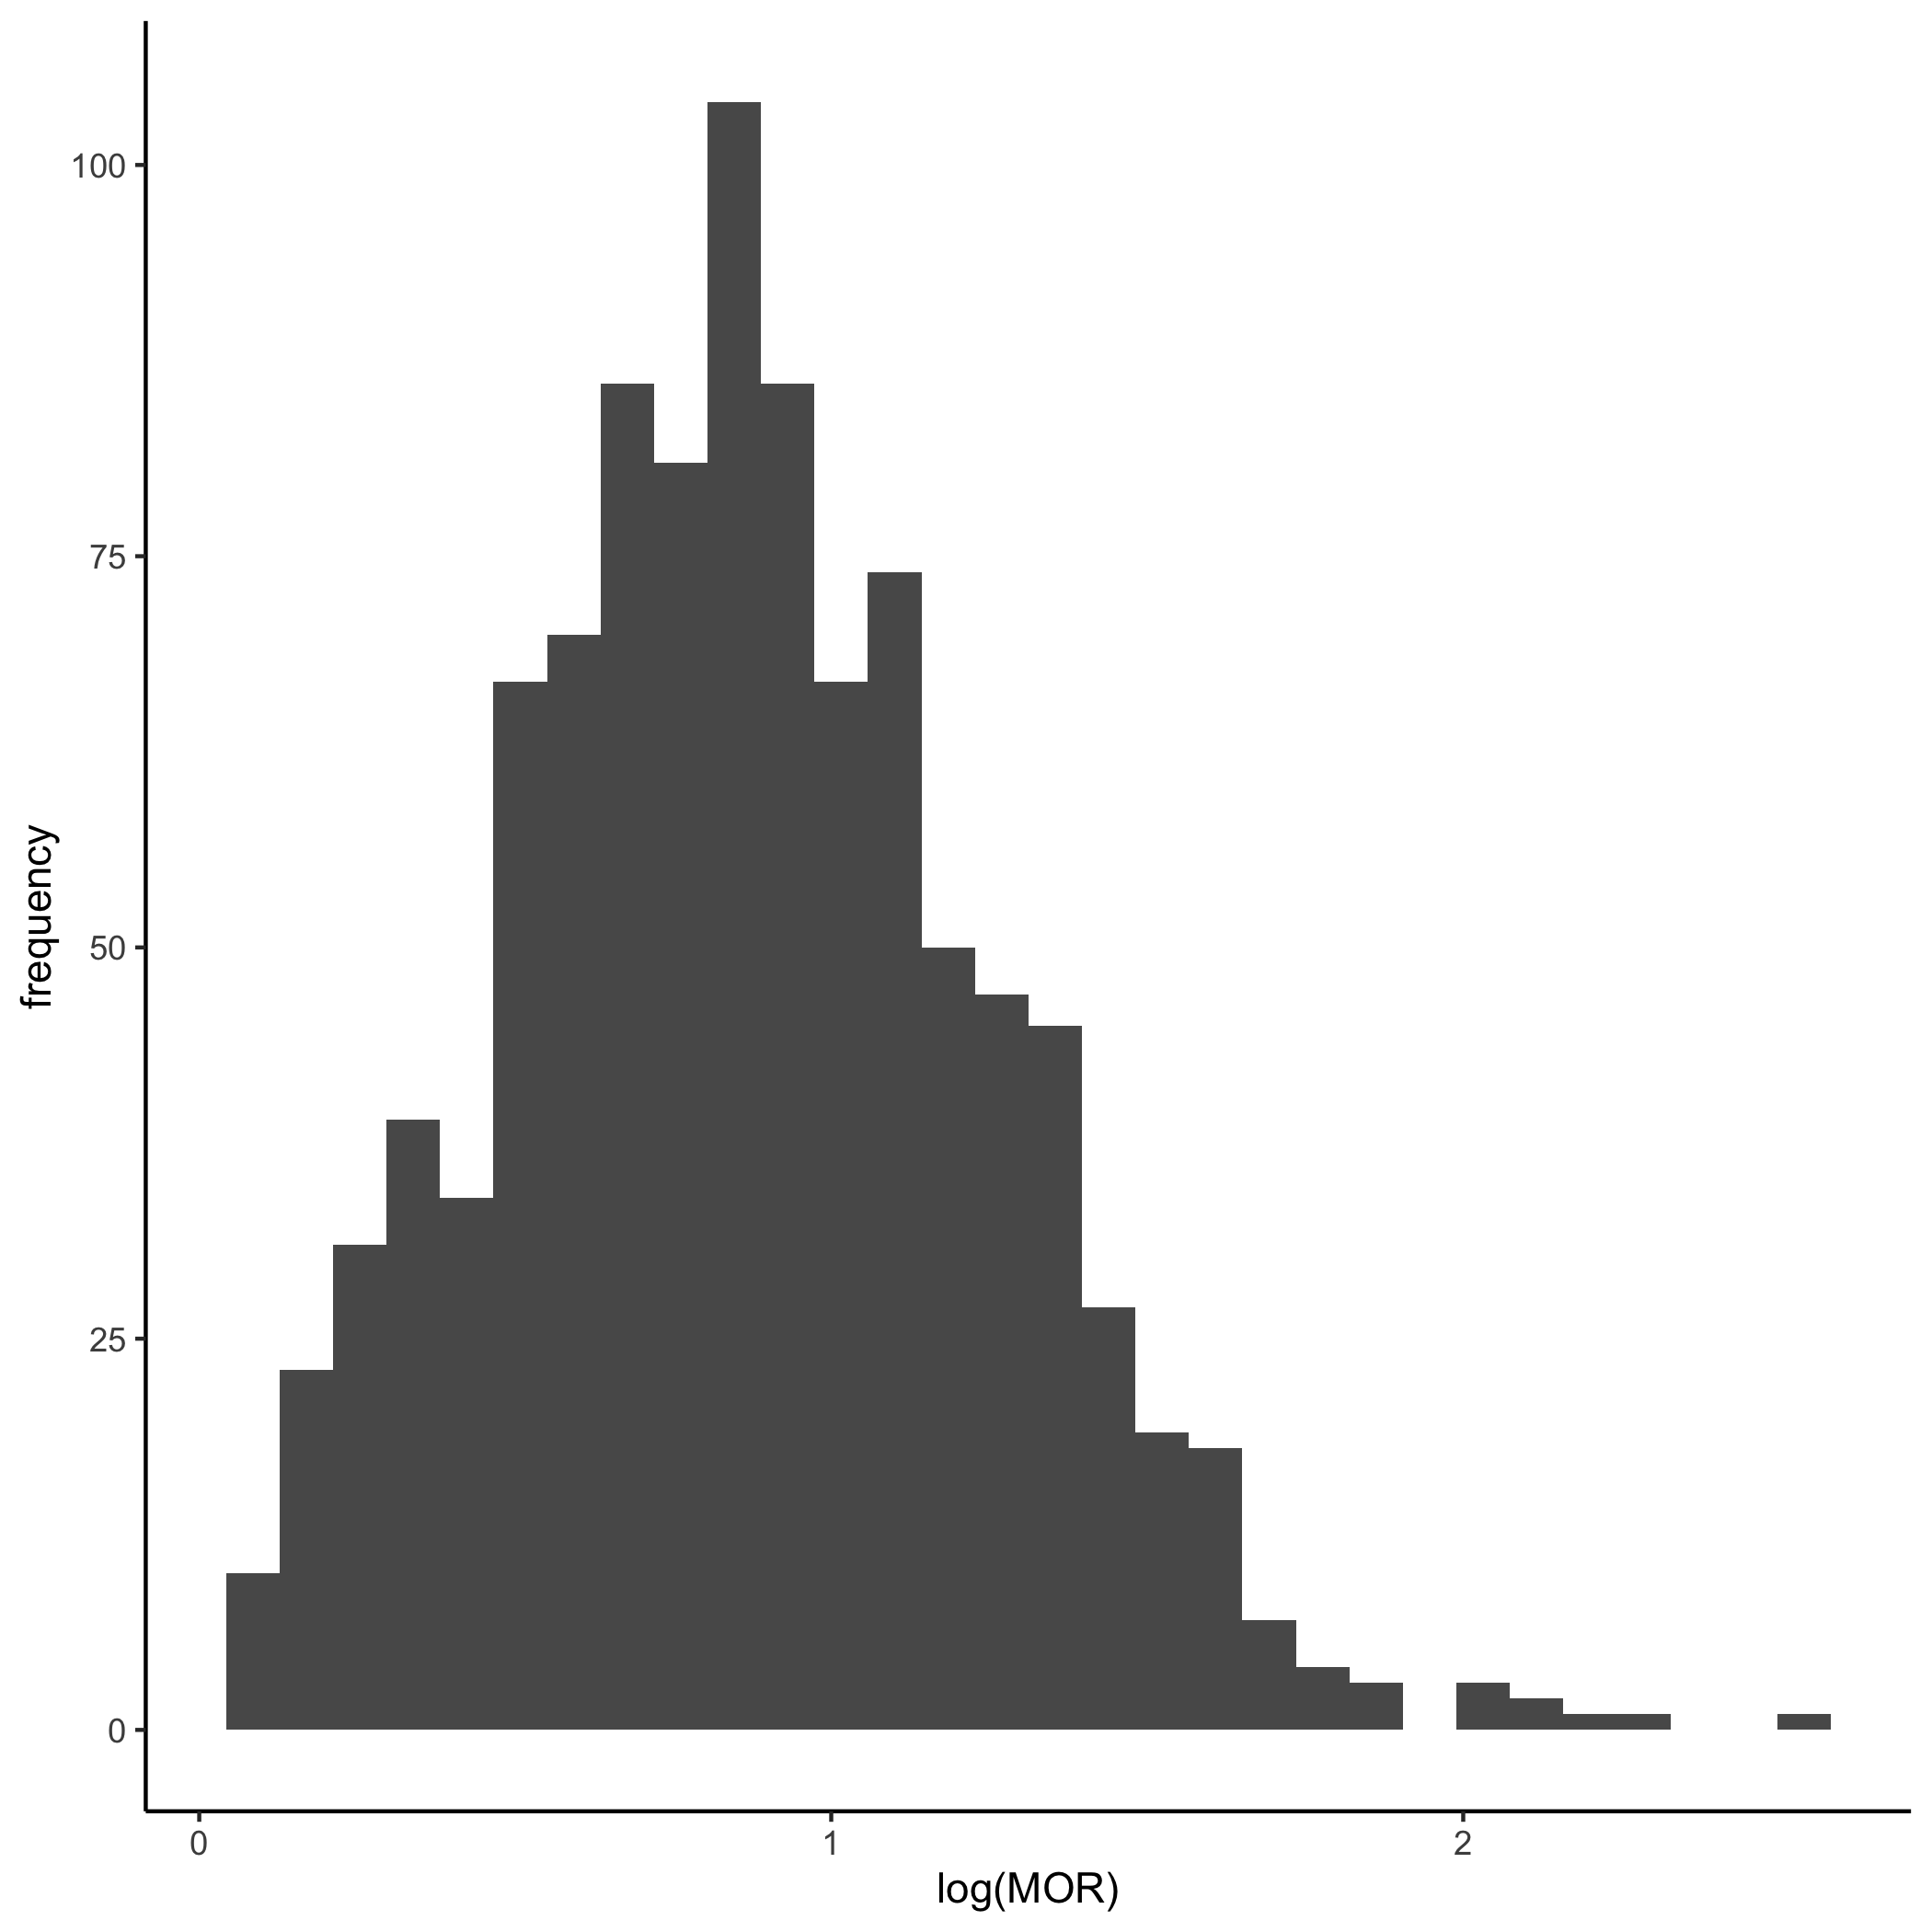
\includegraphics{../../plots/two-lvl-ran-slope/high-prev/hist_10_30_two_lvl_slp_high_prev.png}

}

\caption{For cluster size 30}

}

\end{minipage}%
%
\begin{minipage}[t]{0.50\linewidth}

{\centering 

\raisebox{-\height}{

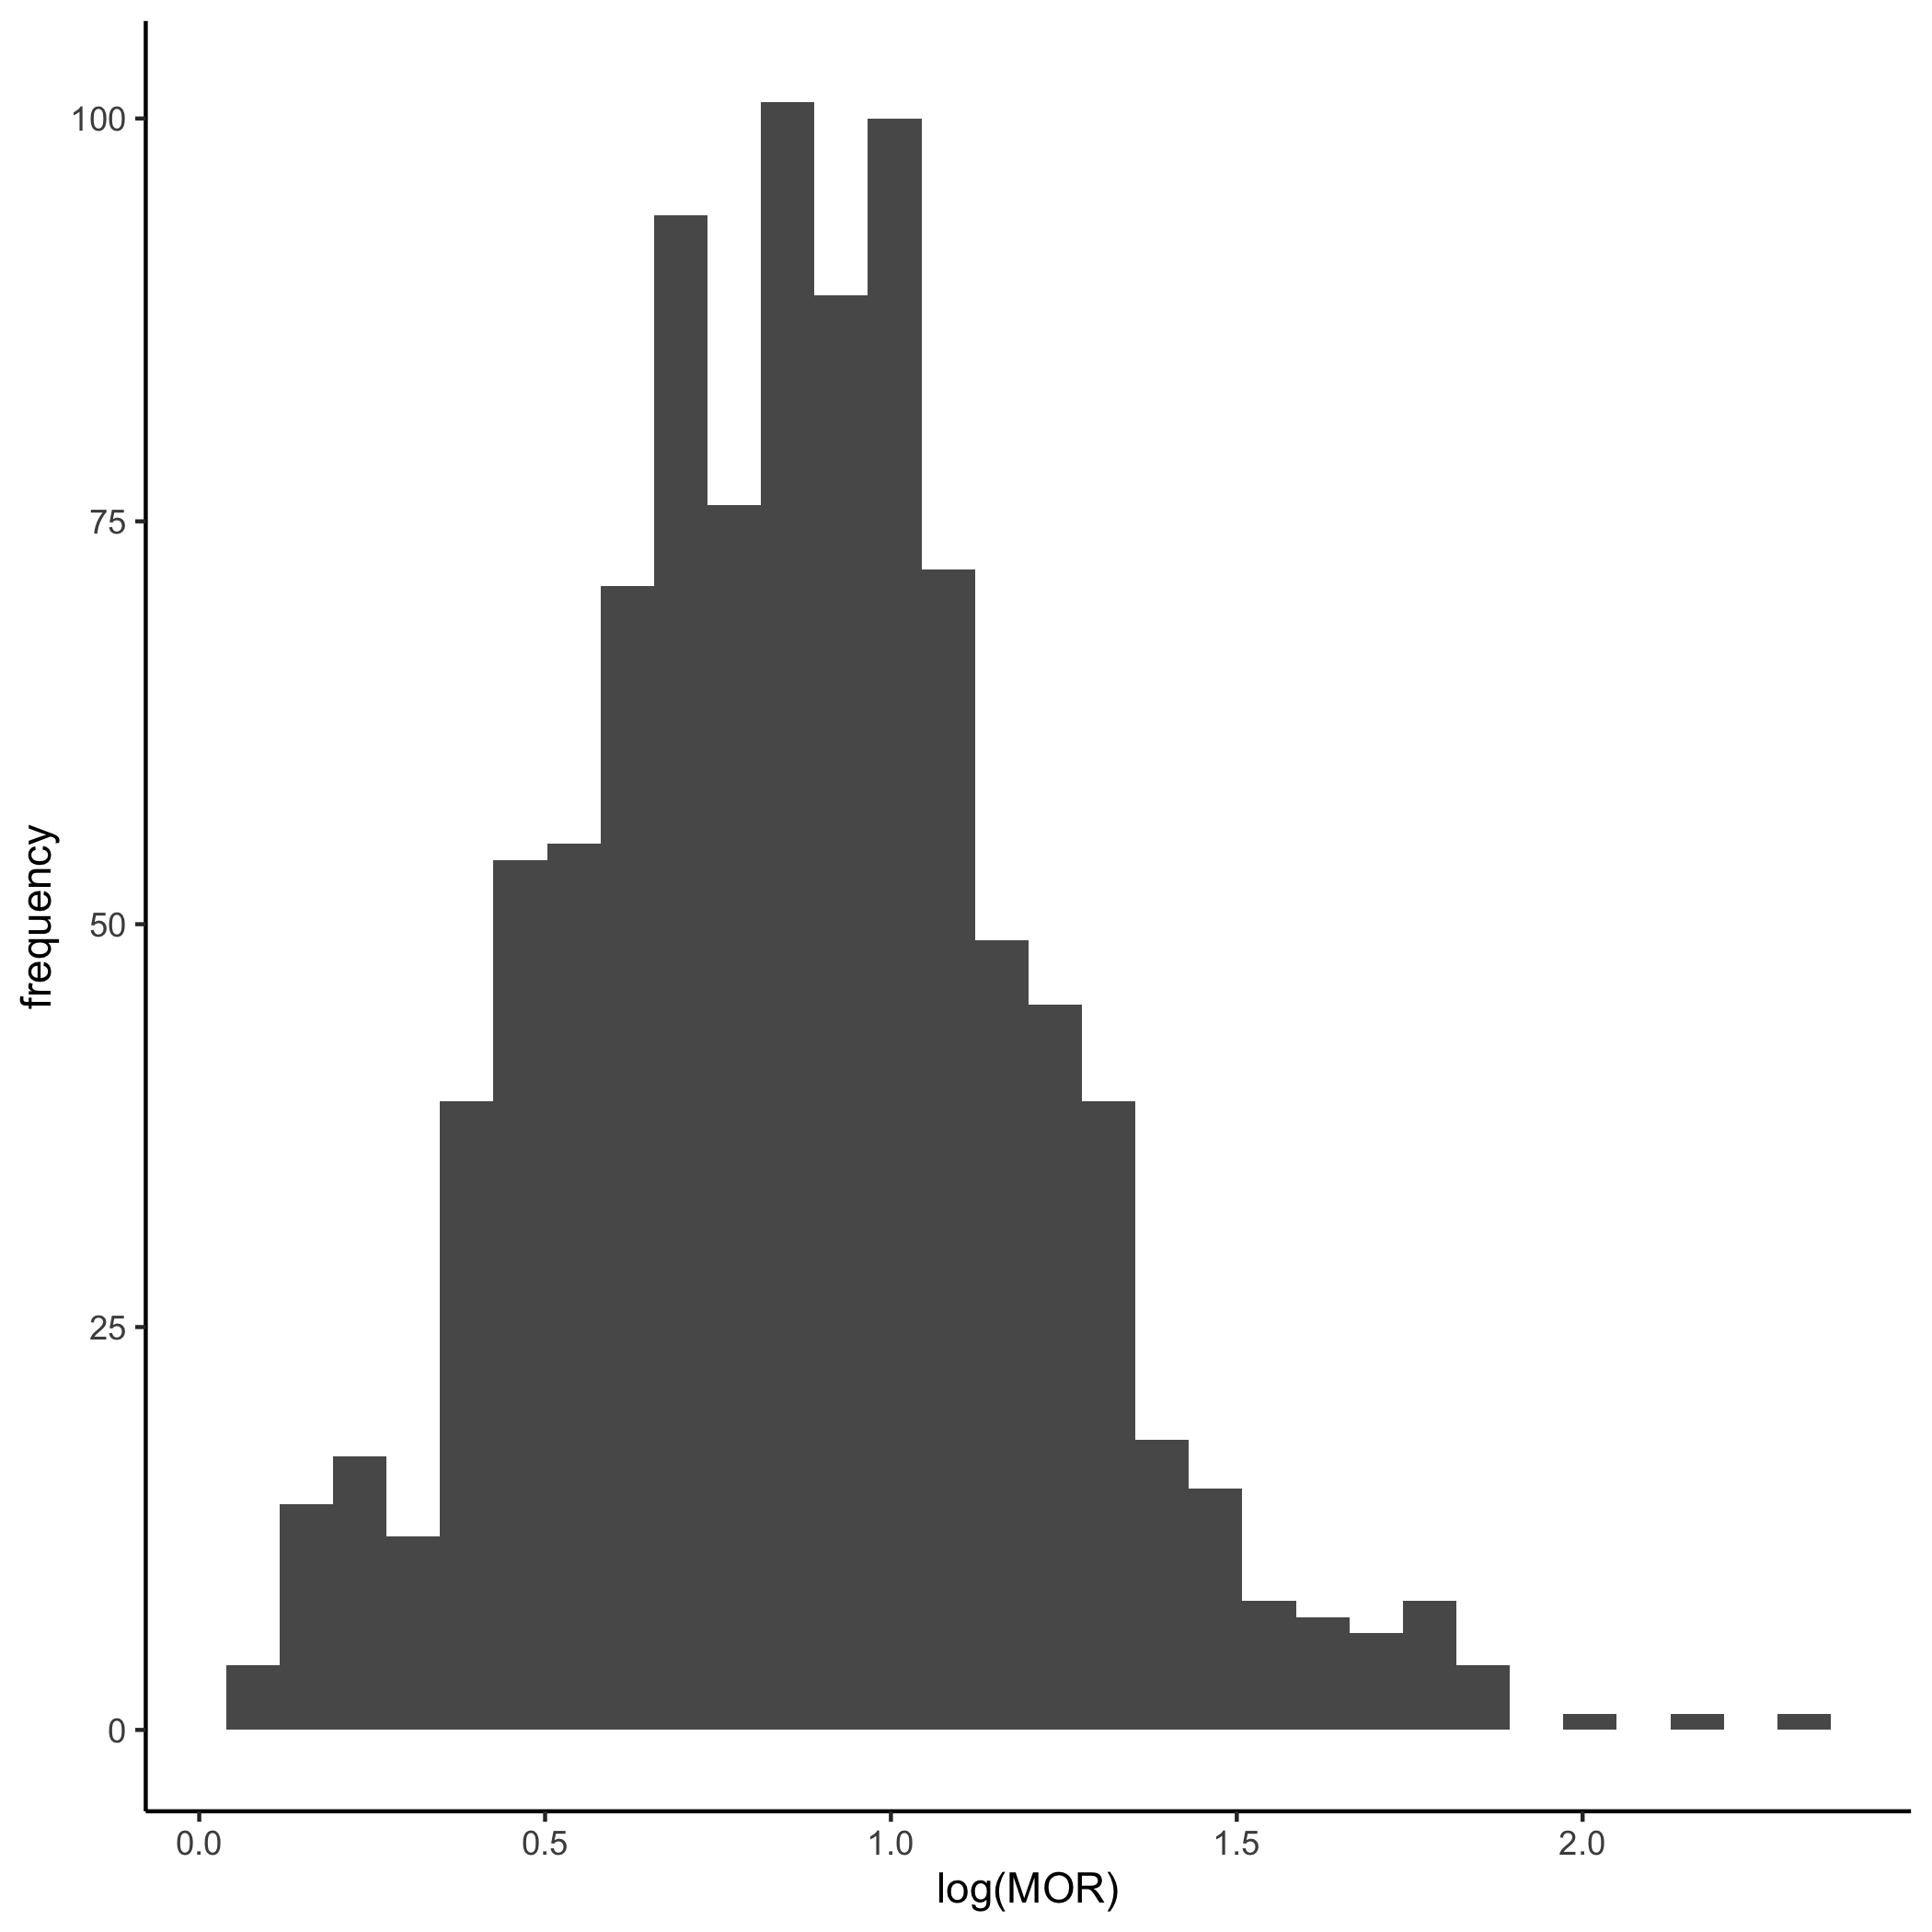
\includegraphics{../../plots/two-lvl-ran-slope/high-prev/hist_10_50_two_lvl_slp_high_prev.png}

}

\caption{For cluster size 50}

}

\end{minipage}%

\end{figure}

\newpage

\hypertarget{histograms-for-logwidehatmor-when-number-of-cluster-is-30}{%
\section{\texorpdfstring{Histograms for \(log(\widehat{MOR})\) When
Number of Cluster is
30}{Histograms for log(\textbackslash widehat\{MOR\}) When Number of Cluster is 30}}\label{histograms-for-logwidehatmor-when-number-of-cluster-is-30}}

\vspace{5mm}

\begin{figure}

\begin{minipage}[t]{0.50\linewidth}

{\centering 

\raisebox{-\height}{

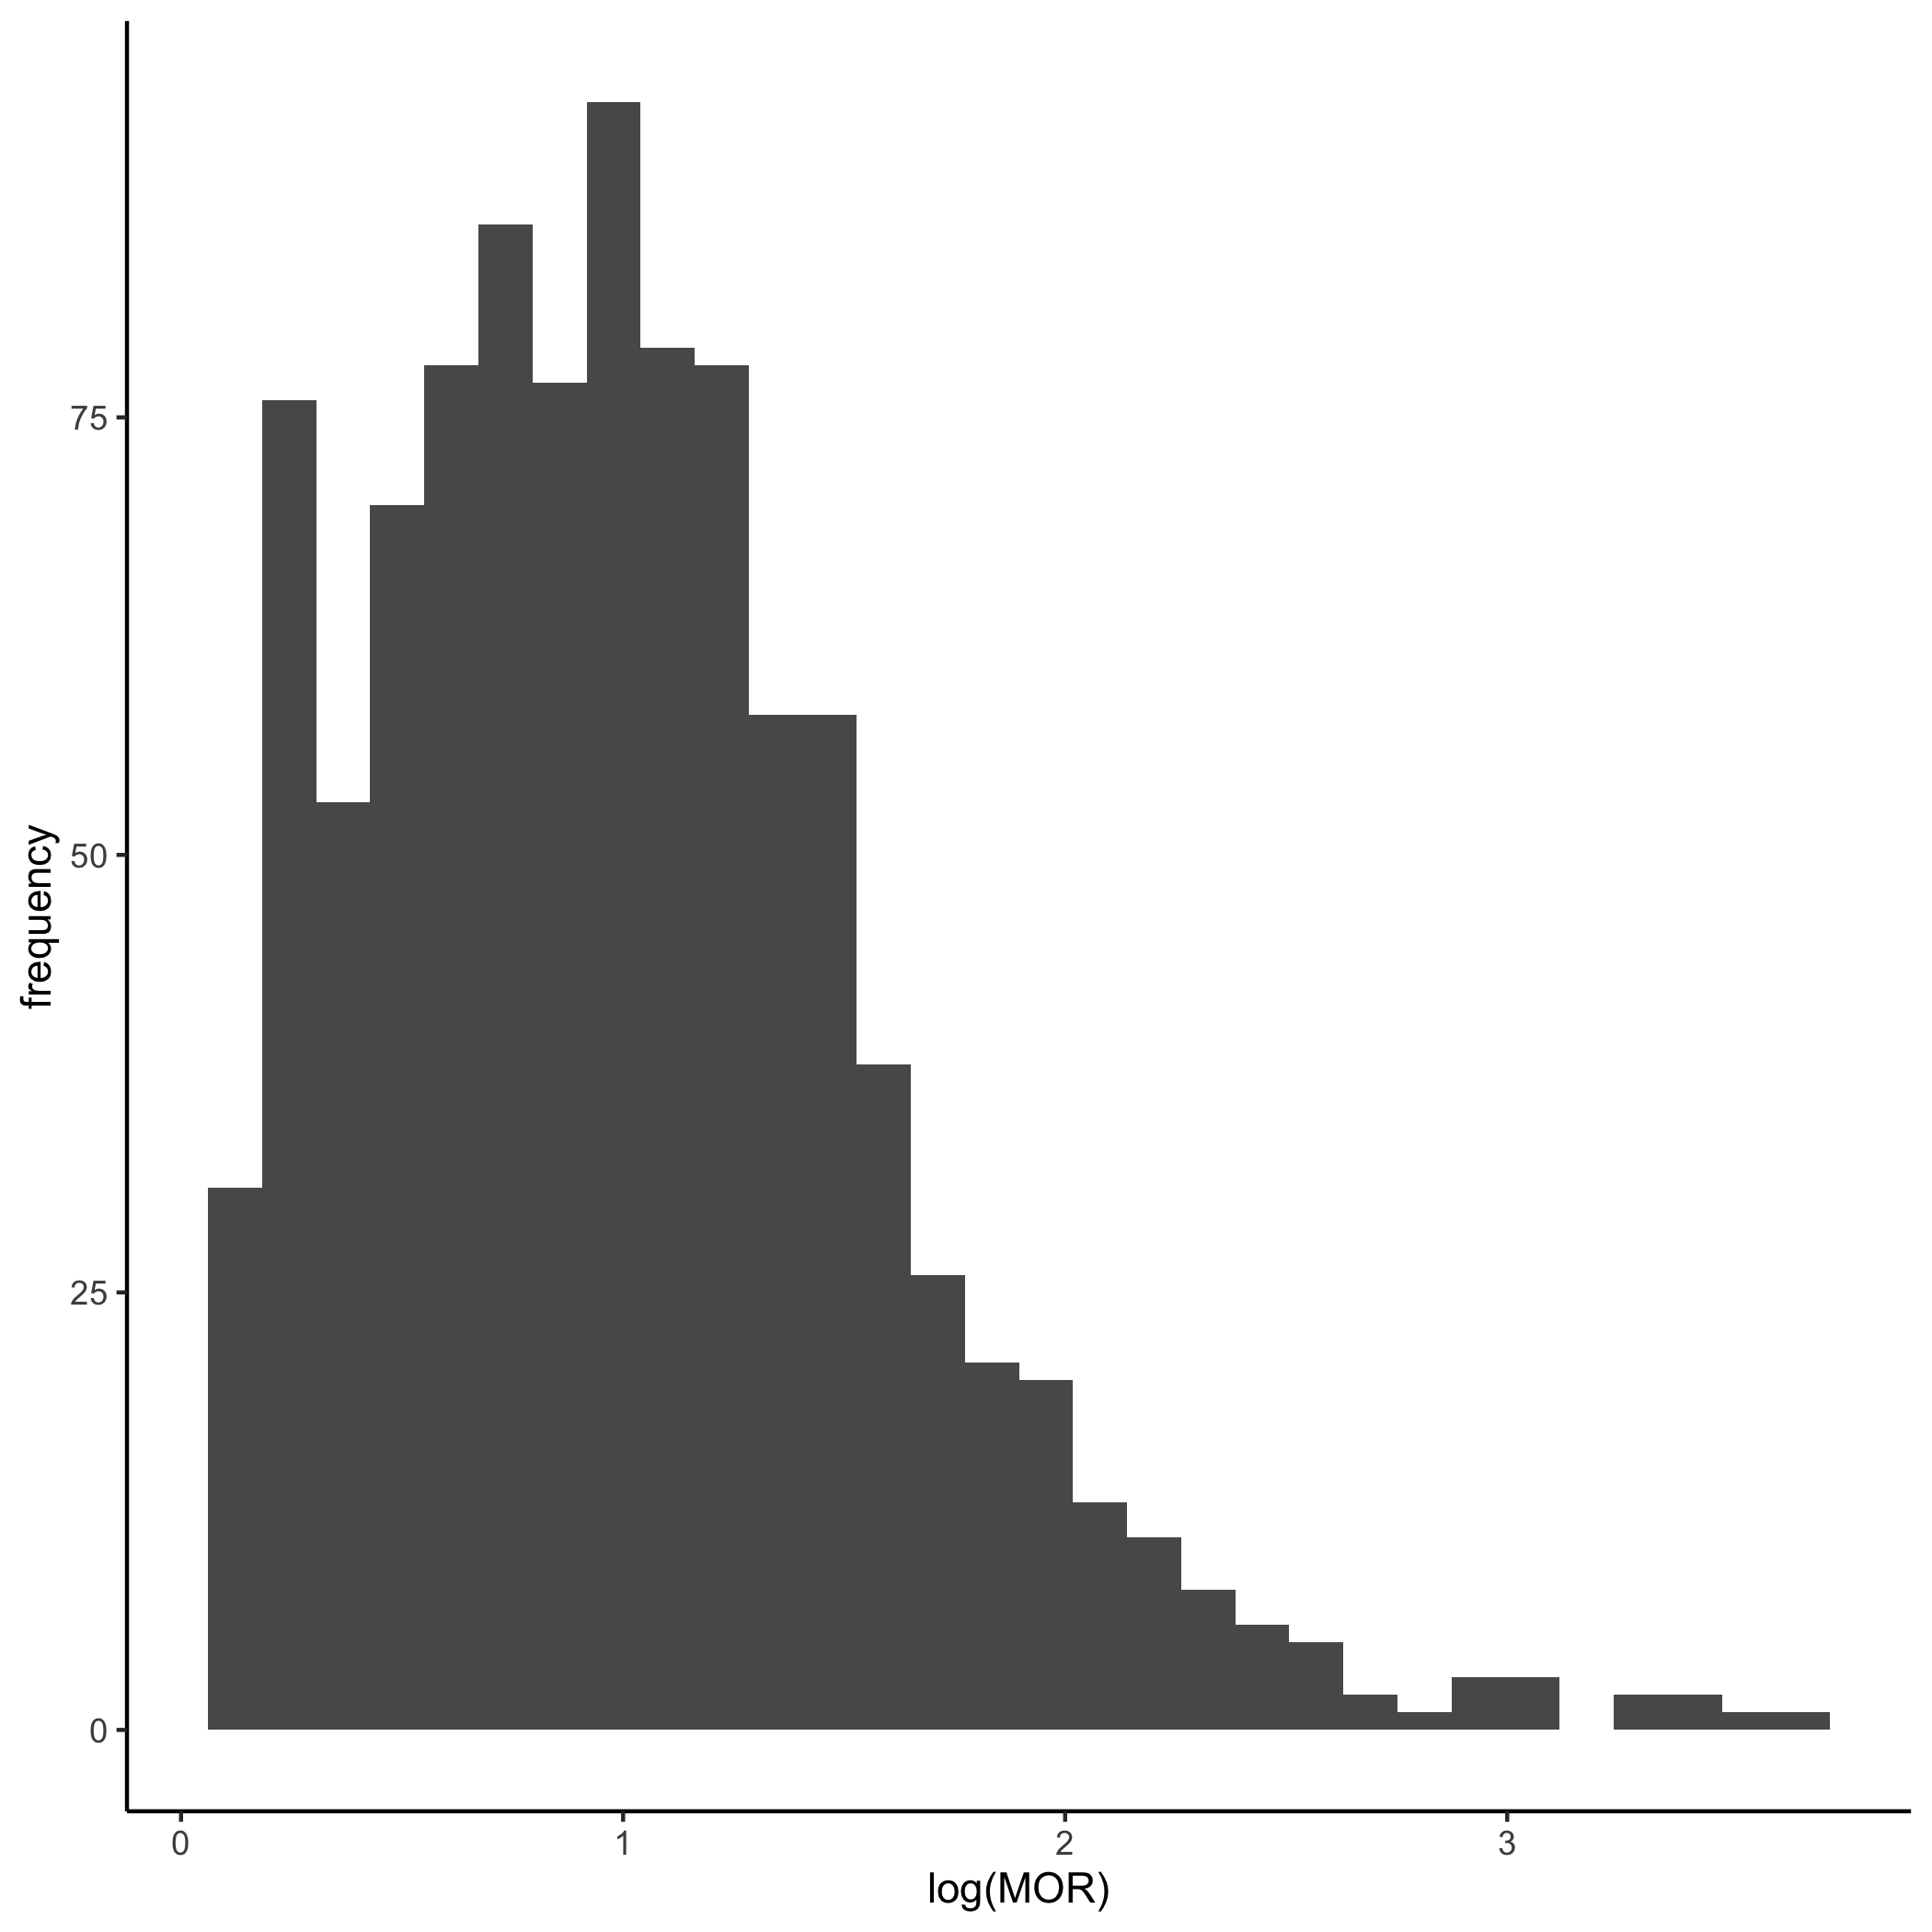
\includegraphics{../../plots/two-lvl-ran-slope/high-prev/hist_30_5_two_lvl_slp_high_prev.png}

}

\caption{For cluster size 5}

}

\end{minipage}%
%
\begin{minipage}[t]{0.50\linewidth}

{\centering 

\raisebox{-\height}{

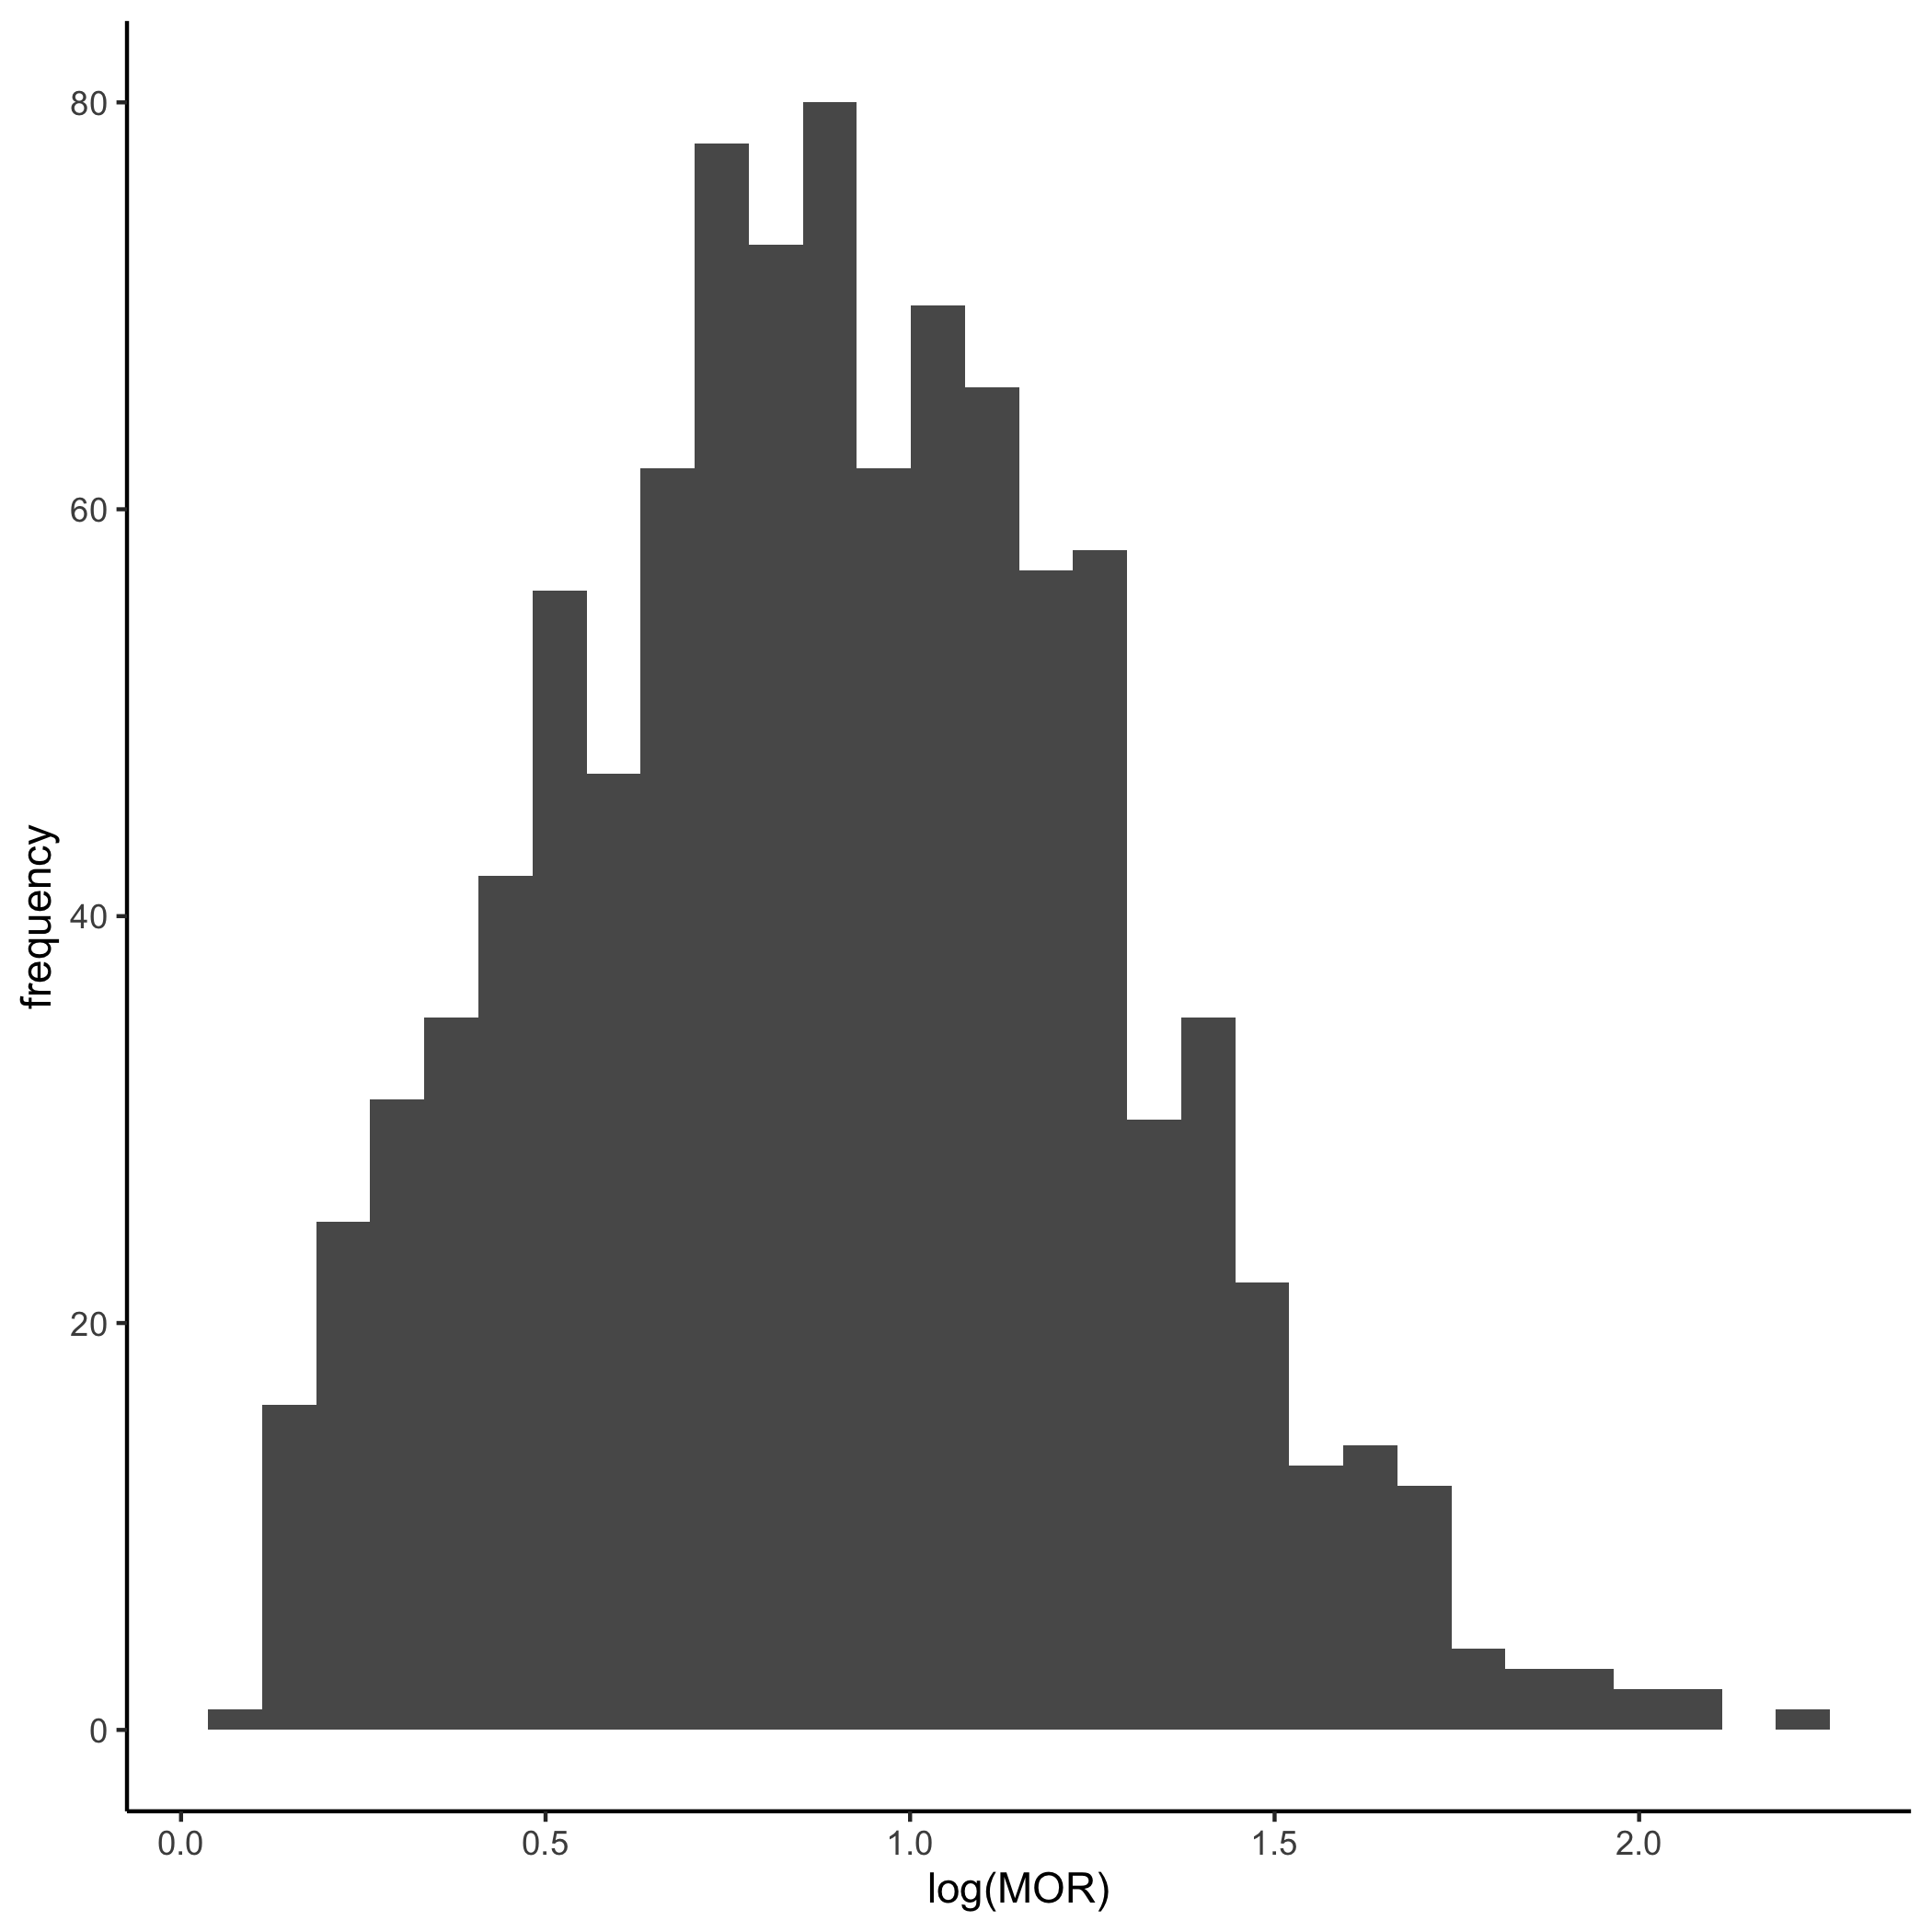
\includegraphics{../../plots/two-lvl-ran-slope/high-prev/hist_30_10_two_lvl_slp_high_prev.png}

}

\caption{For cluster size 10}

}

\end{minipage}%
\newline
\begin{minipage}[t]{\linewidth}

{\centering 

~

}

\end{minipage}%
\newline
\begin{minipage}[t]{0.50\linewidth}

{\centering 

\raisebox{-\height}{

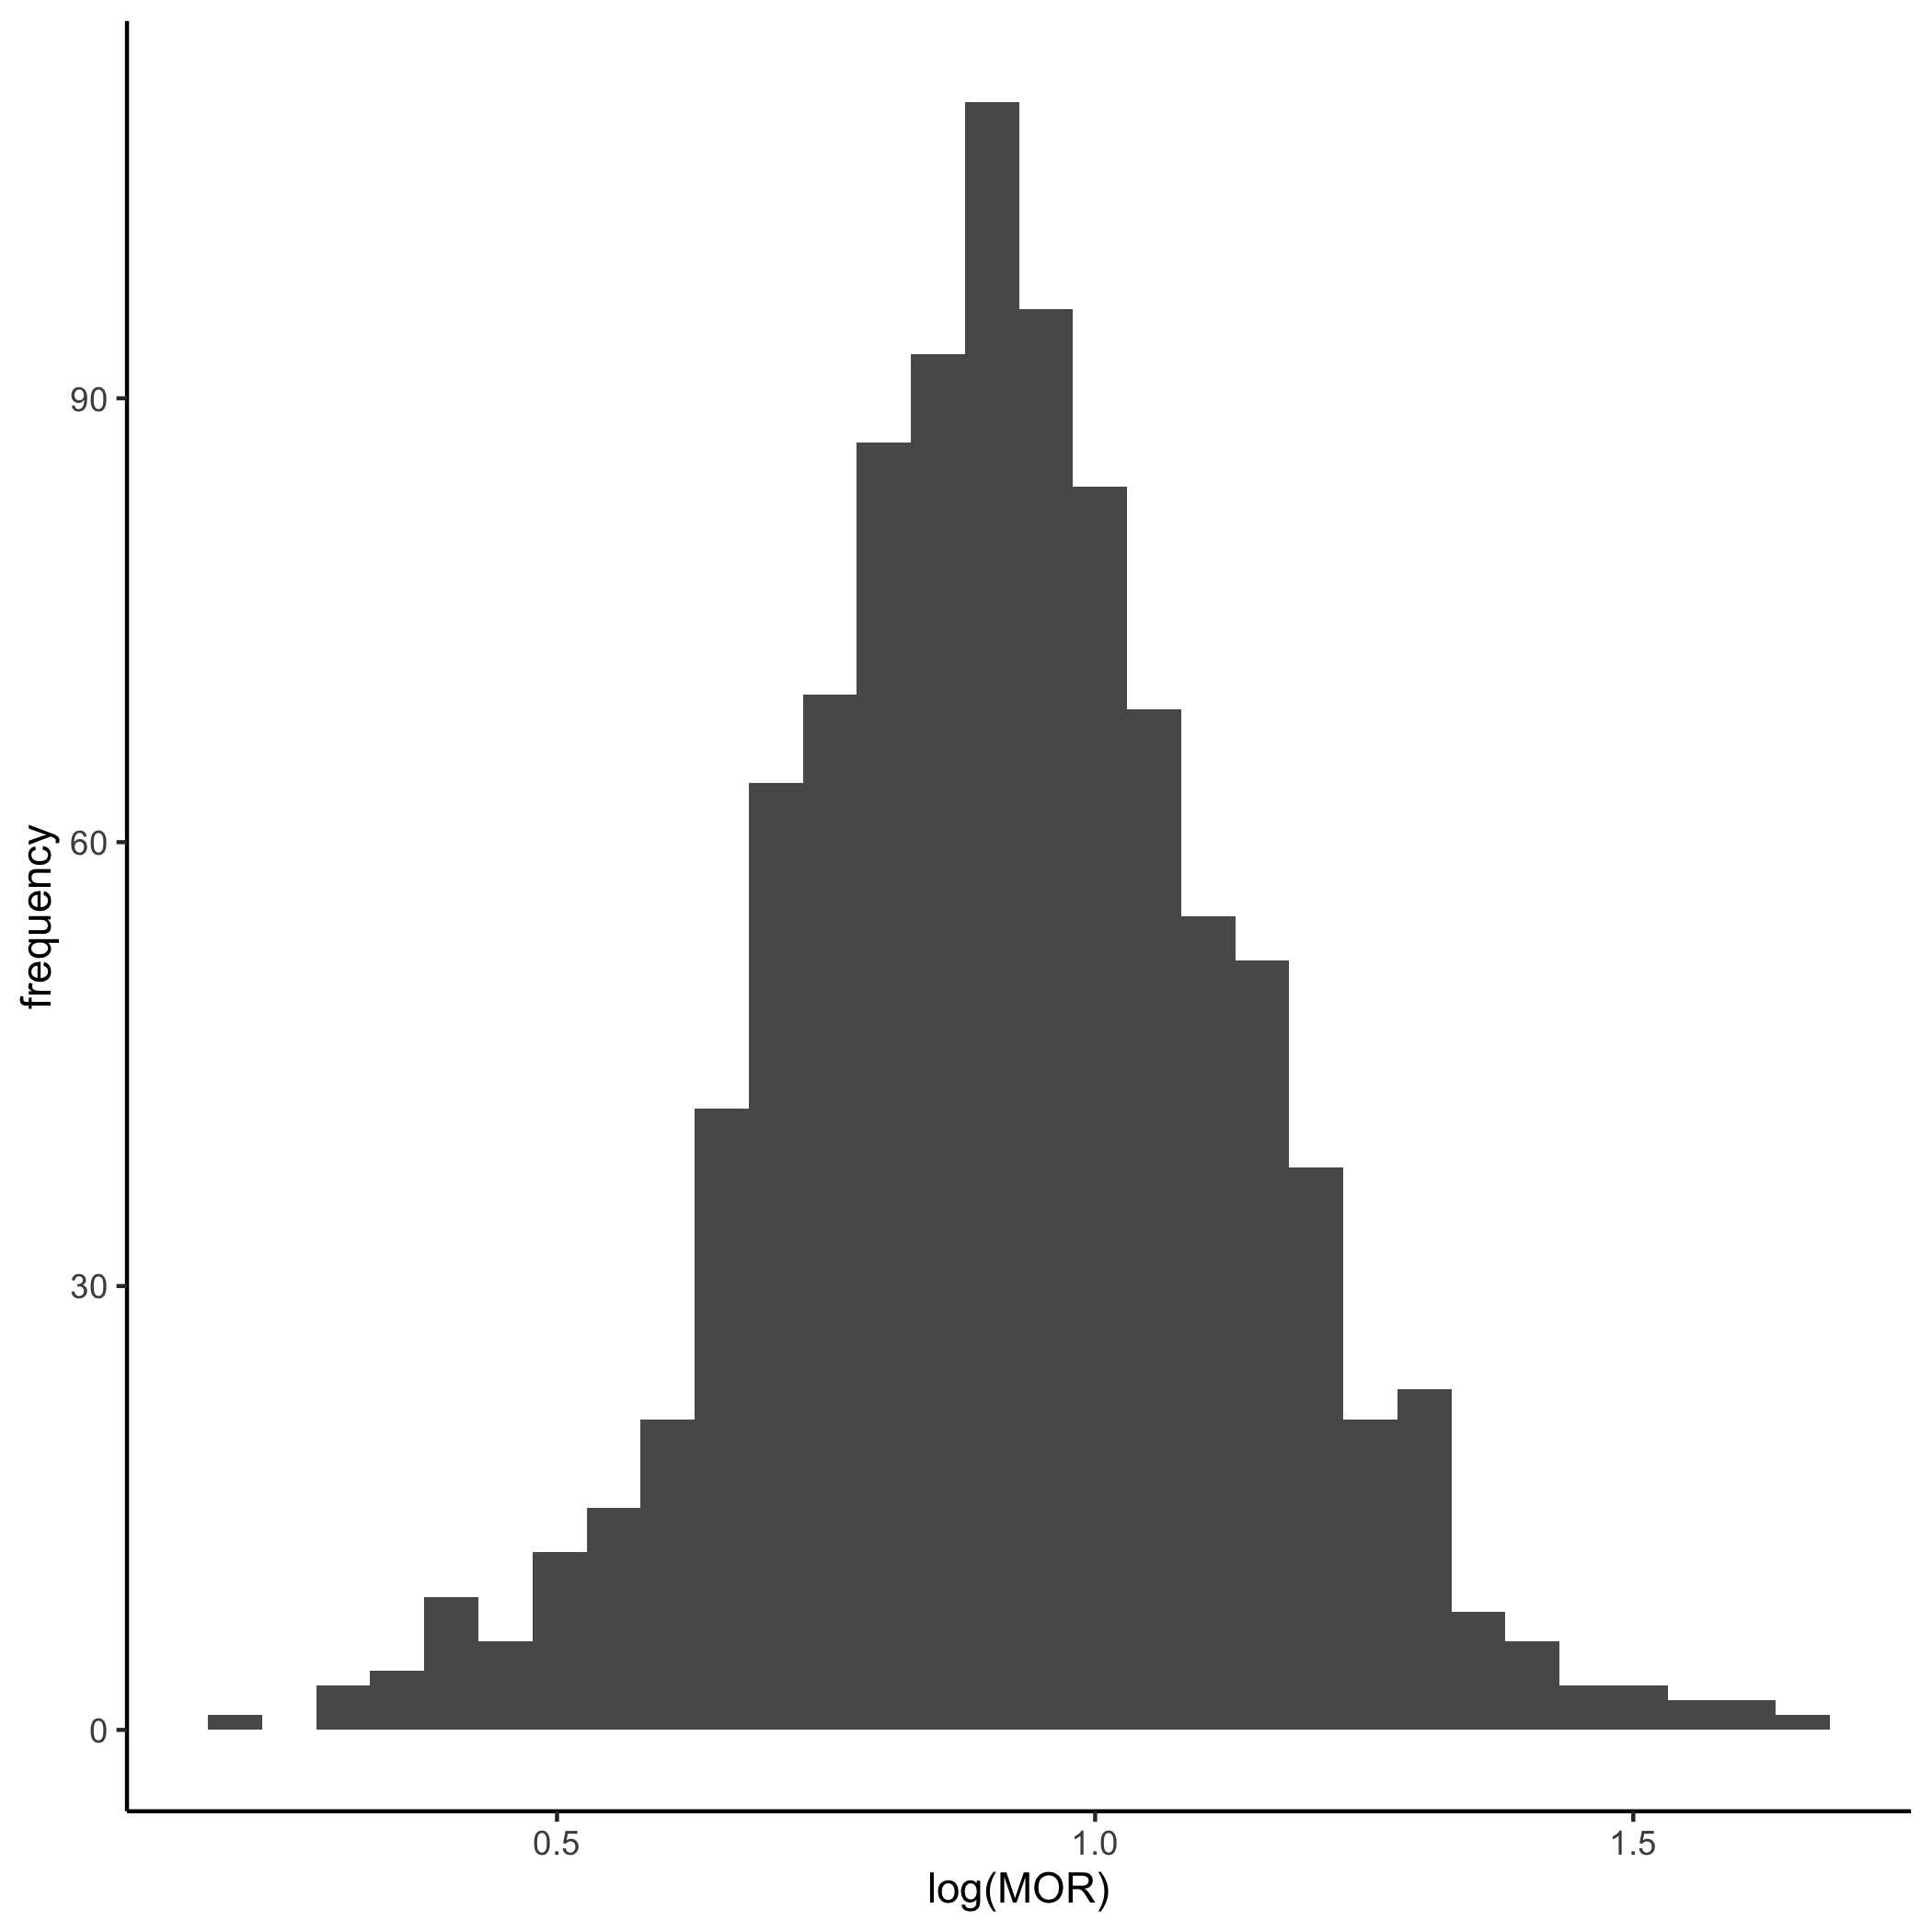
\includegraphics{../../plots/two-lvl-ran-slope/high-prev/hist_30_30_two_lvl_slp_high_prev.png}

}

\caption{For cluster size 30}

}

\end{minipage}%
%
\begin{minipage}[t]{0.50\linewidth}

{\centering 

\raisebox{-\height}{

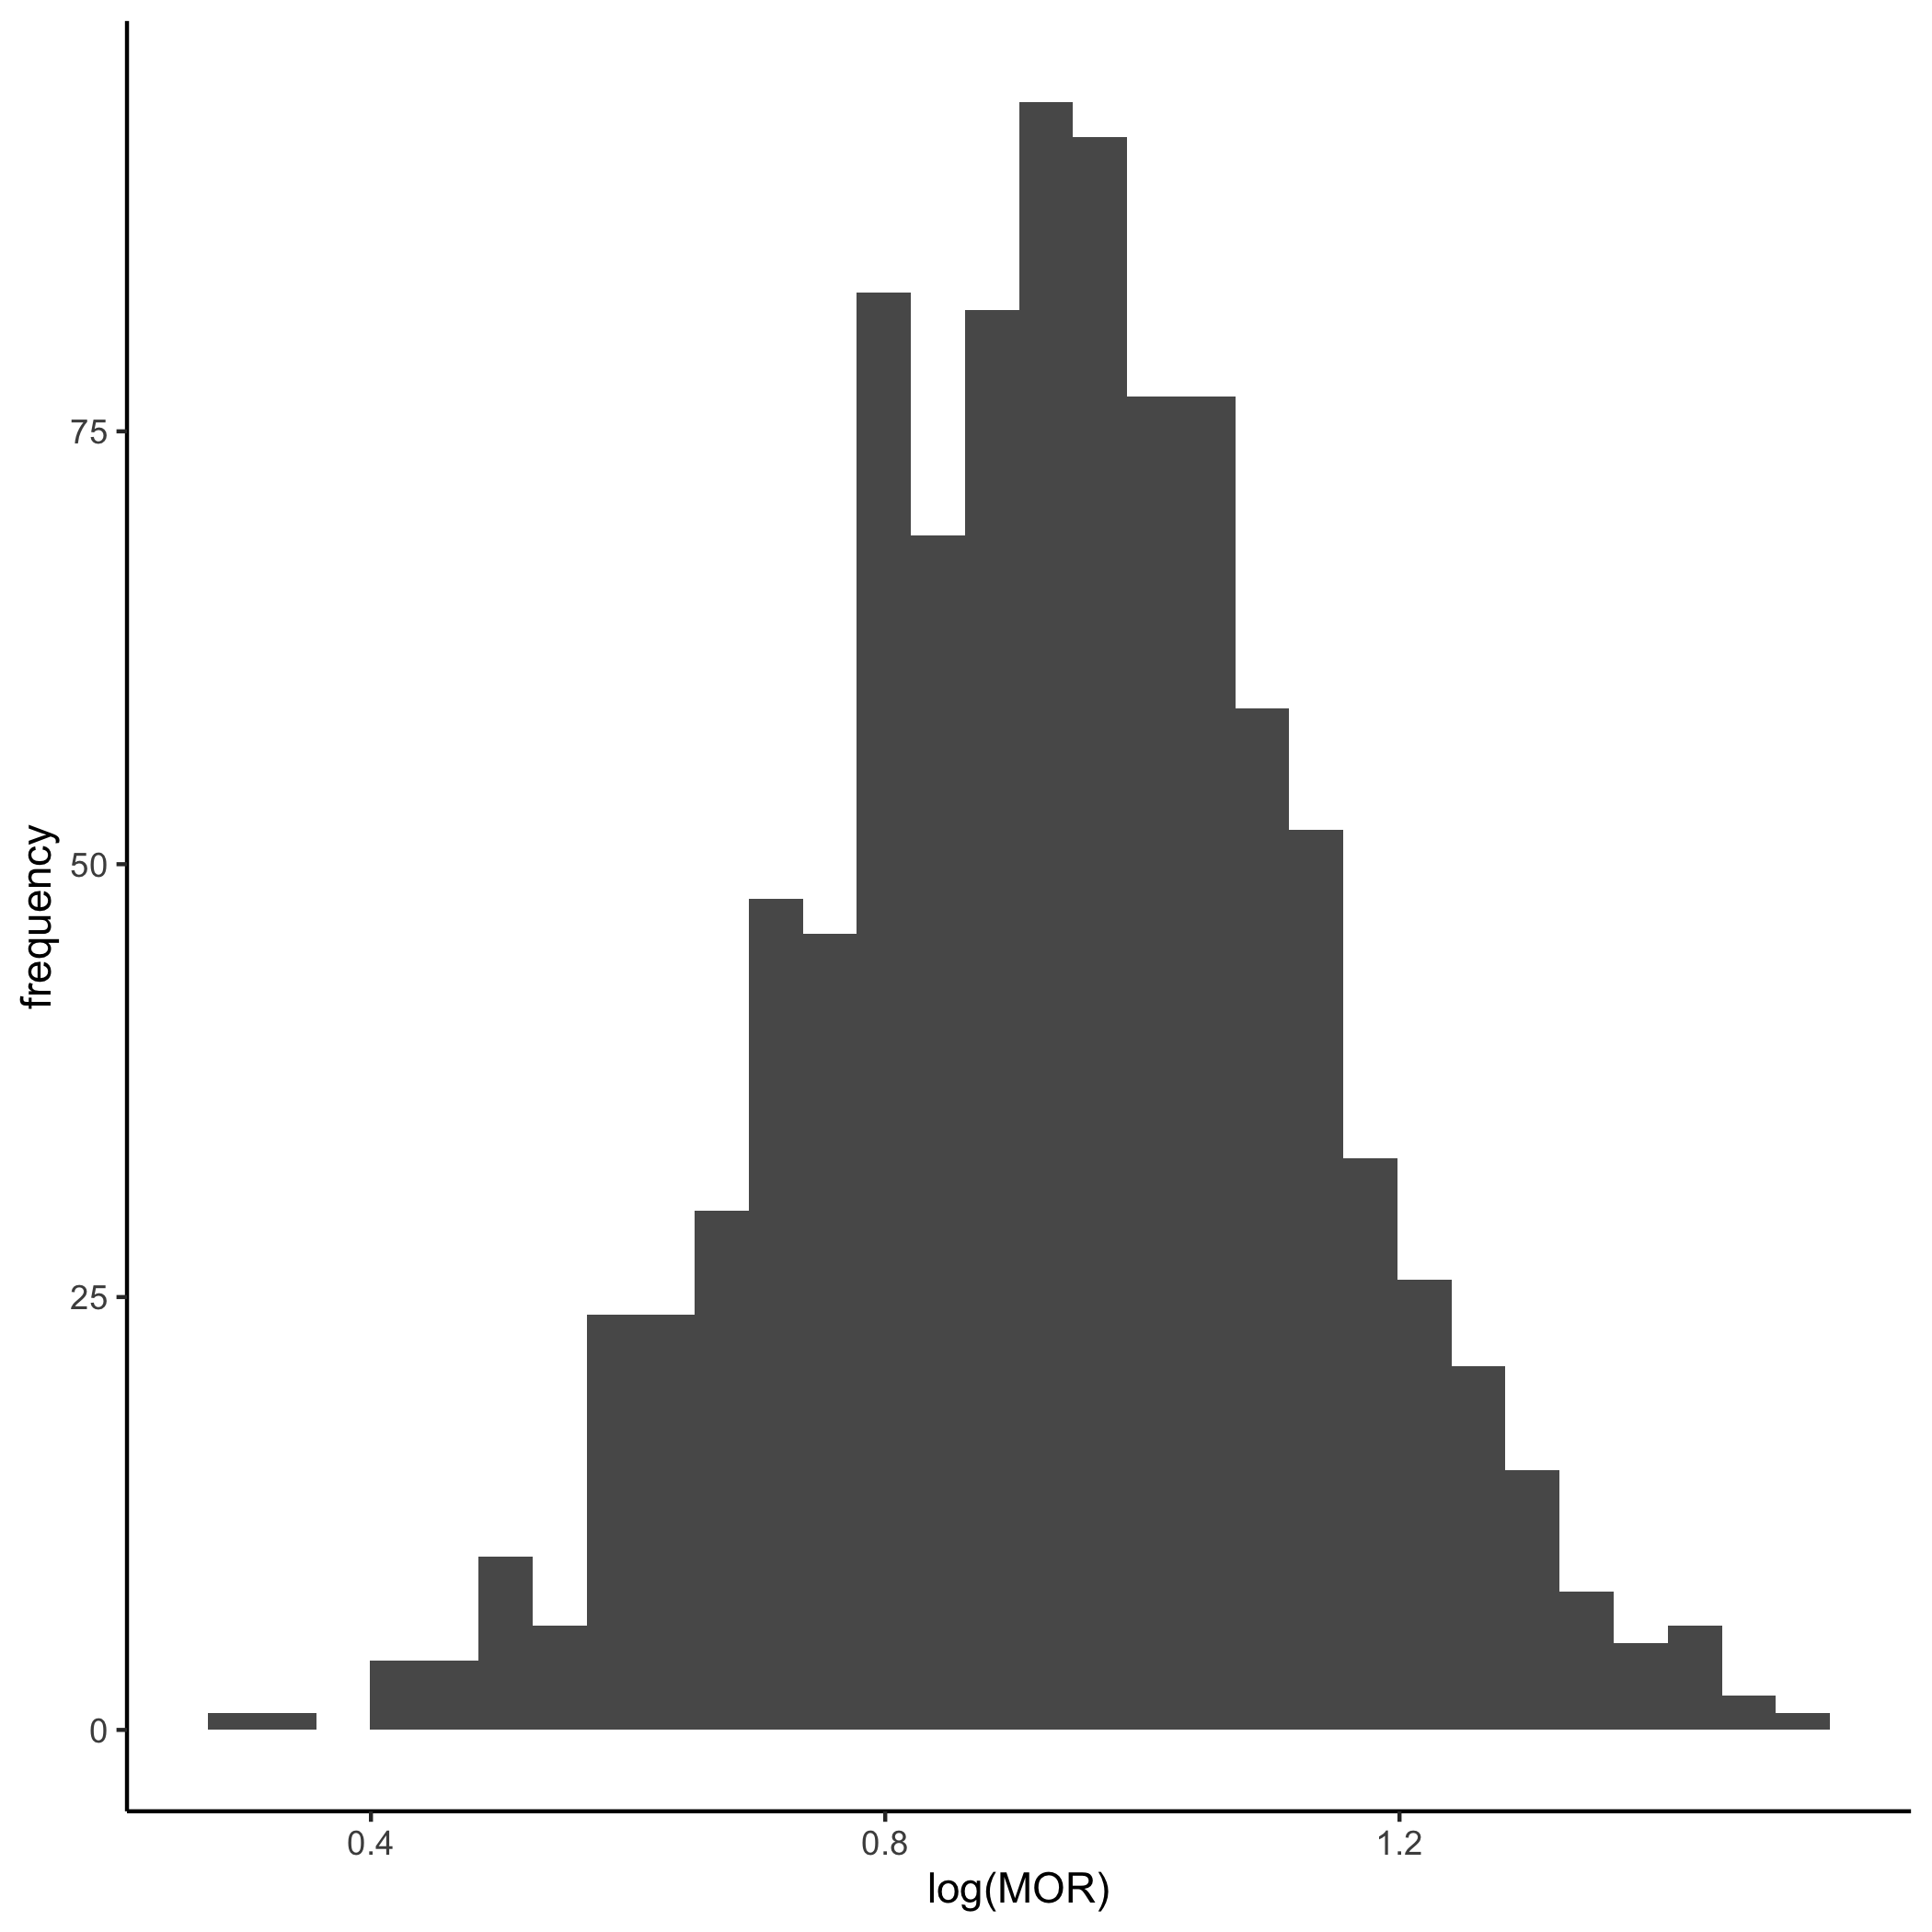
\includegraphics{../../plots/two-lvl-ran-slope/high-prev/hist_30_50_two_lvl_slp_high_prev.png}

}

\caption{For cluster size 50}

}

\end{minipage}%

\end{figure}

\newpage

\hypertarget{histograms-for-logwidehatmor-when-number-of-cluster-is-50}{%
\section{\texorpdfstring{Histograms for \(log(\widehat{MOR})\) When
Number of Cluster is
50}{Histograms for log(\textbackslash widehat\{MOR\}) When Number of Cluster is 50}}\label{histograms-for-logwidehatmor-when-number-of-cluster-is-50}}

\vspace{5mm}

\begin{figure}

\begin{minipage}[t]{0.50\linewidth}

{\centering 

\raisebox{-\height}{

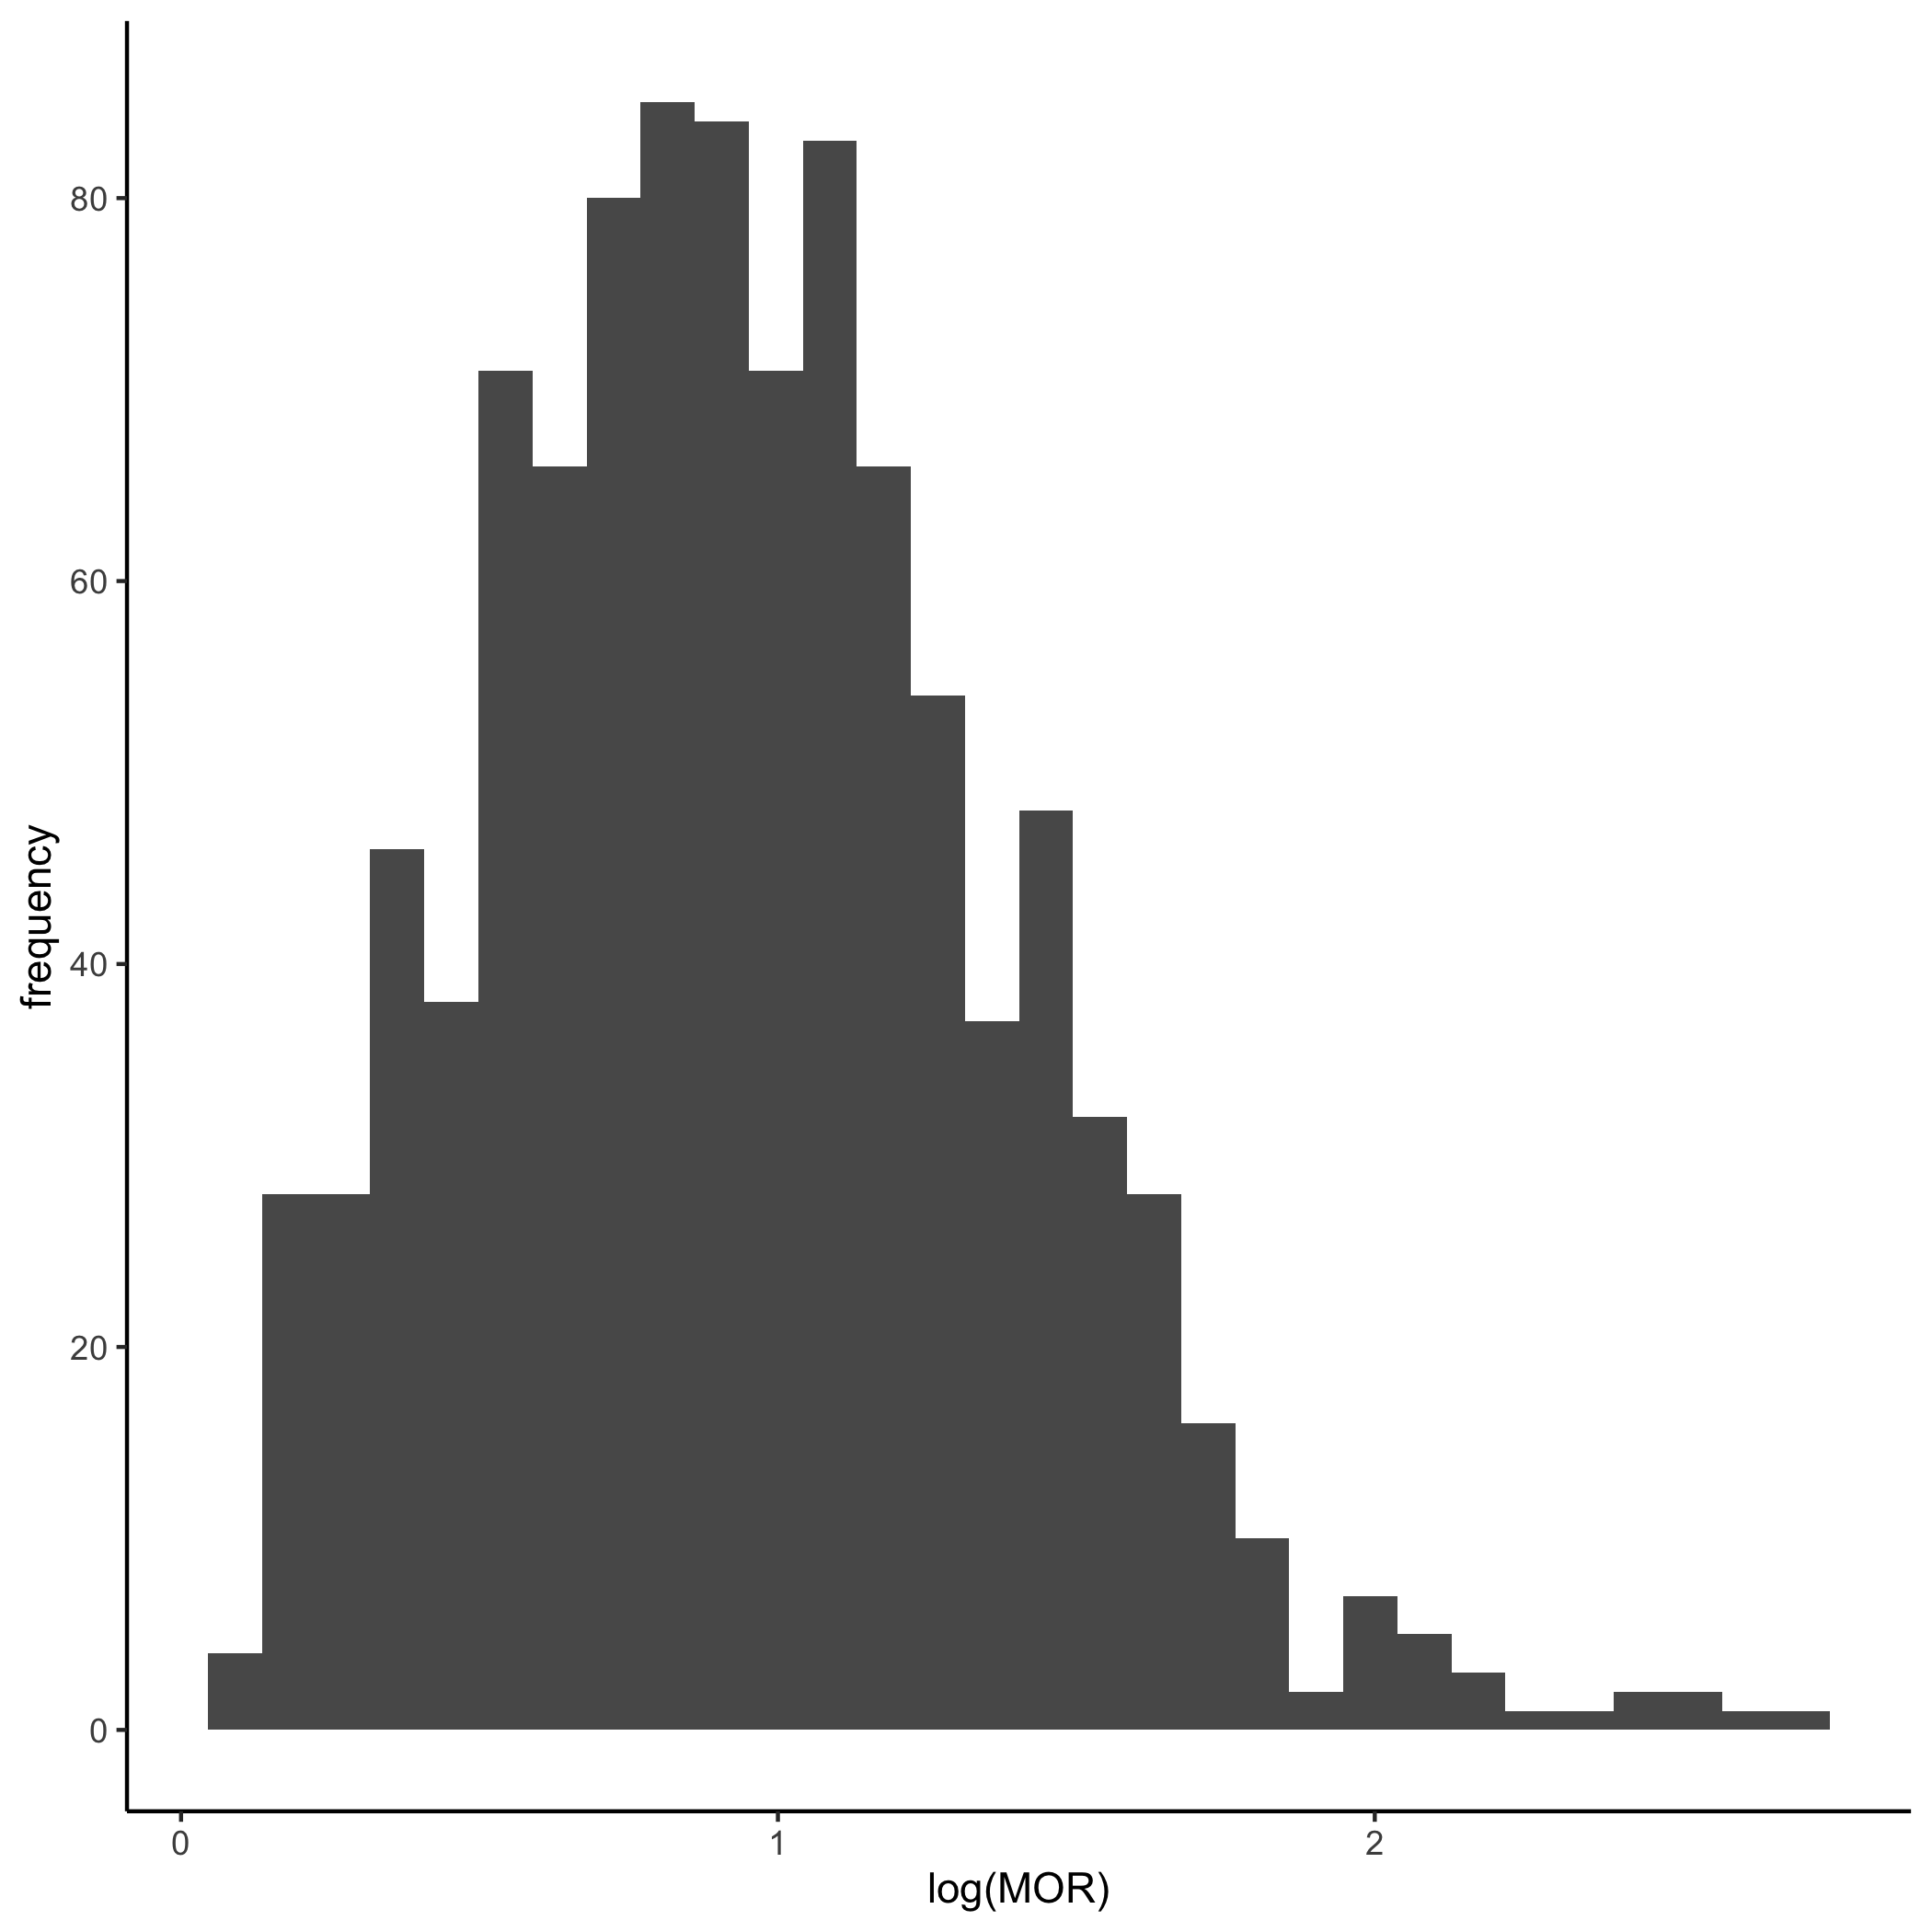
\includegraphics{../../plots/two-lvl-ran-slope/high-prev/hist_50_5_two_lvl_slp_high_prev.png}

}

\caption{For cluster size 5}

}

\end{minipage}%
%
\begin{minipage}[t]{0.50\linewidth}

{\centering 

\raisebox{-\height}{

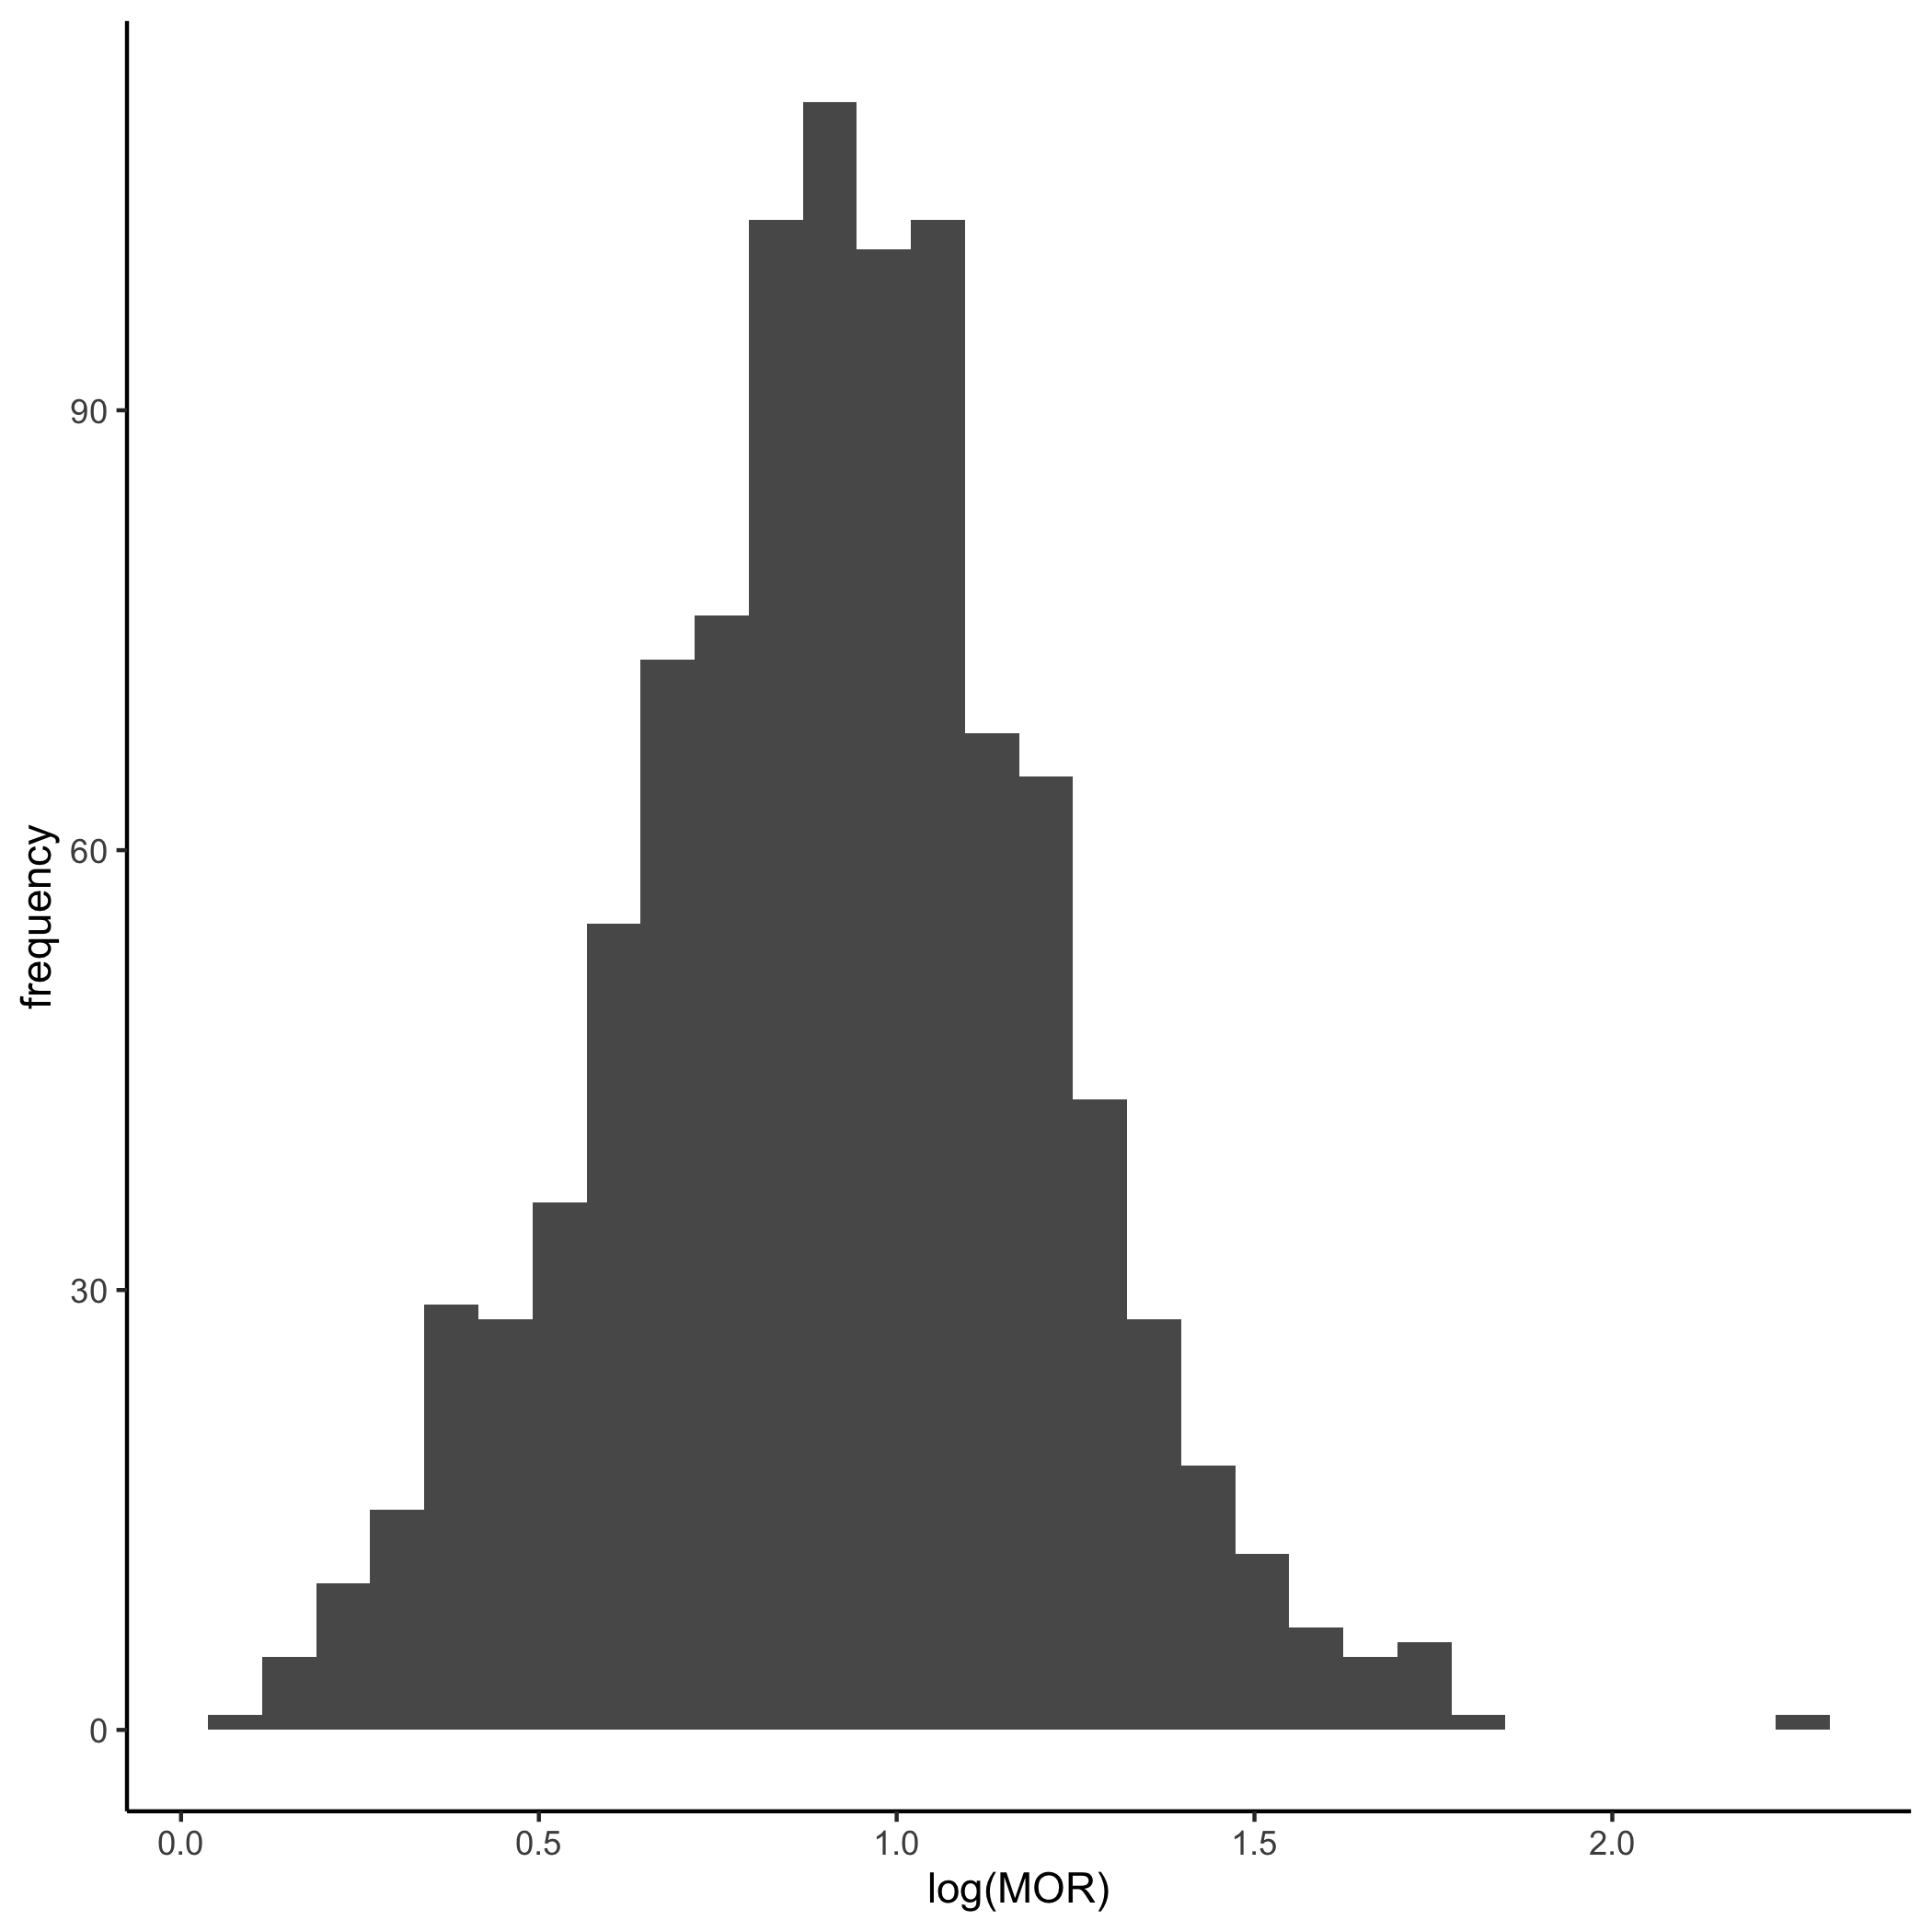
\includegraphics{../../plots/two-lvl-ran-slope/high-prev/hist_50_10_two_lvl_slp_high_prev.png}

}

\caption{For cluster size 10}

}

\end{minipage}%
\newline
\begin{minipage}[t]{\linewidth}

{\centering 

~

}

\end{minipage}%
\newline
\begin{minipage}[t]{0.50\linewidth}

{\centering 

\raisebox{-\height}{

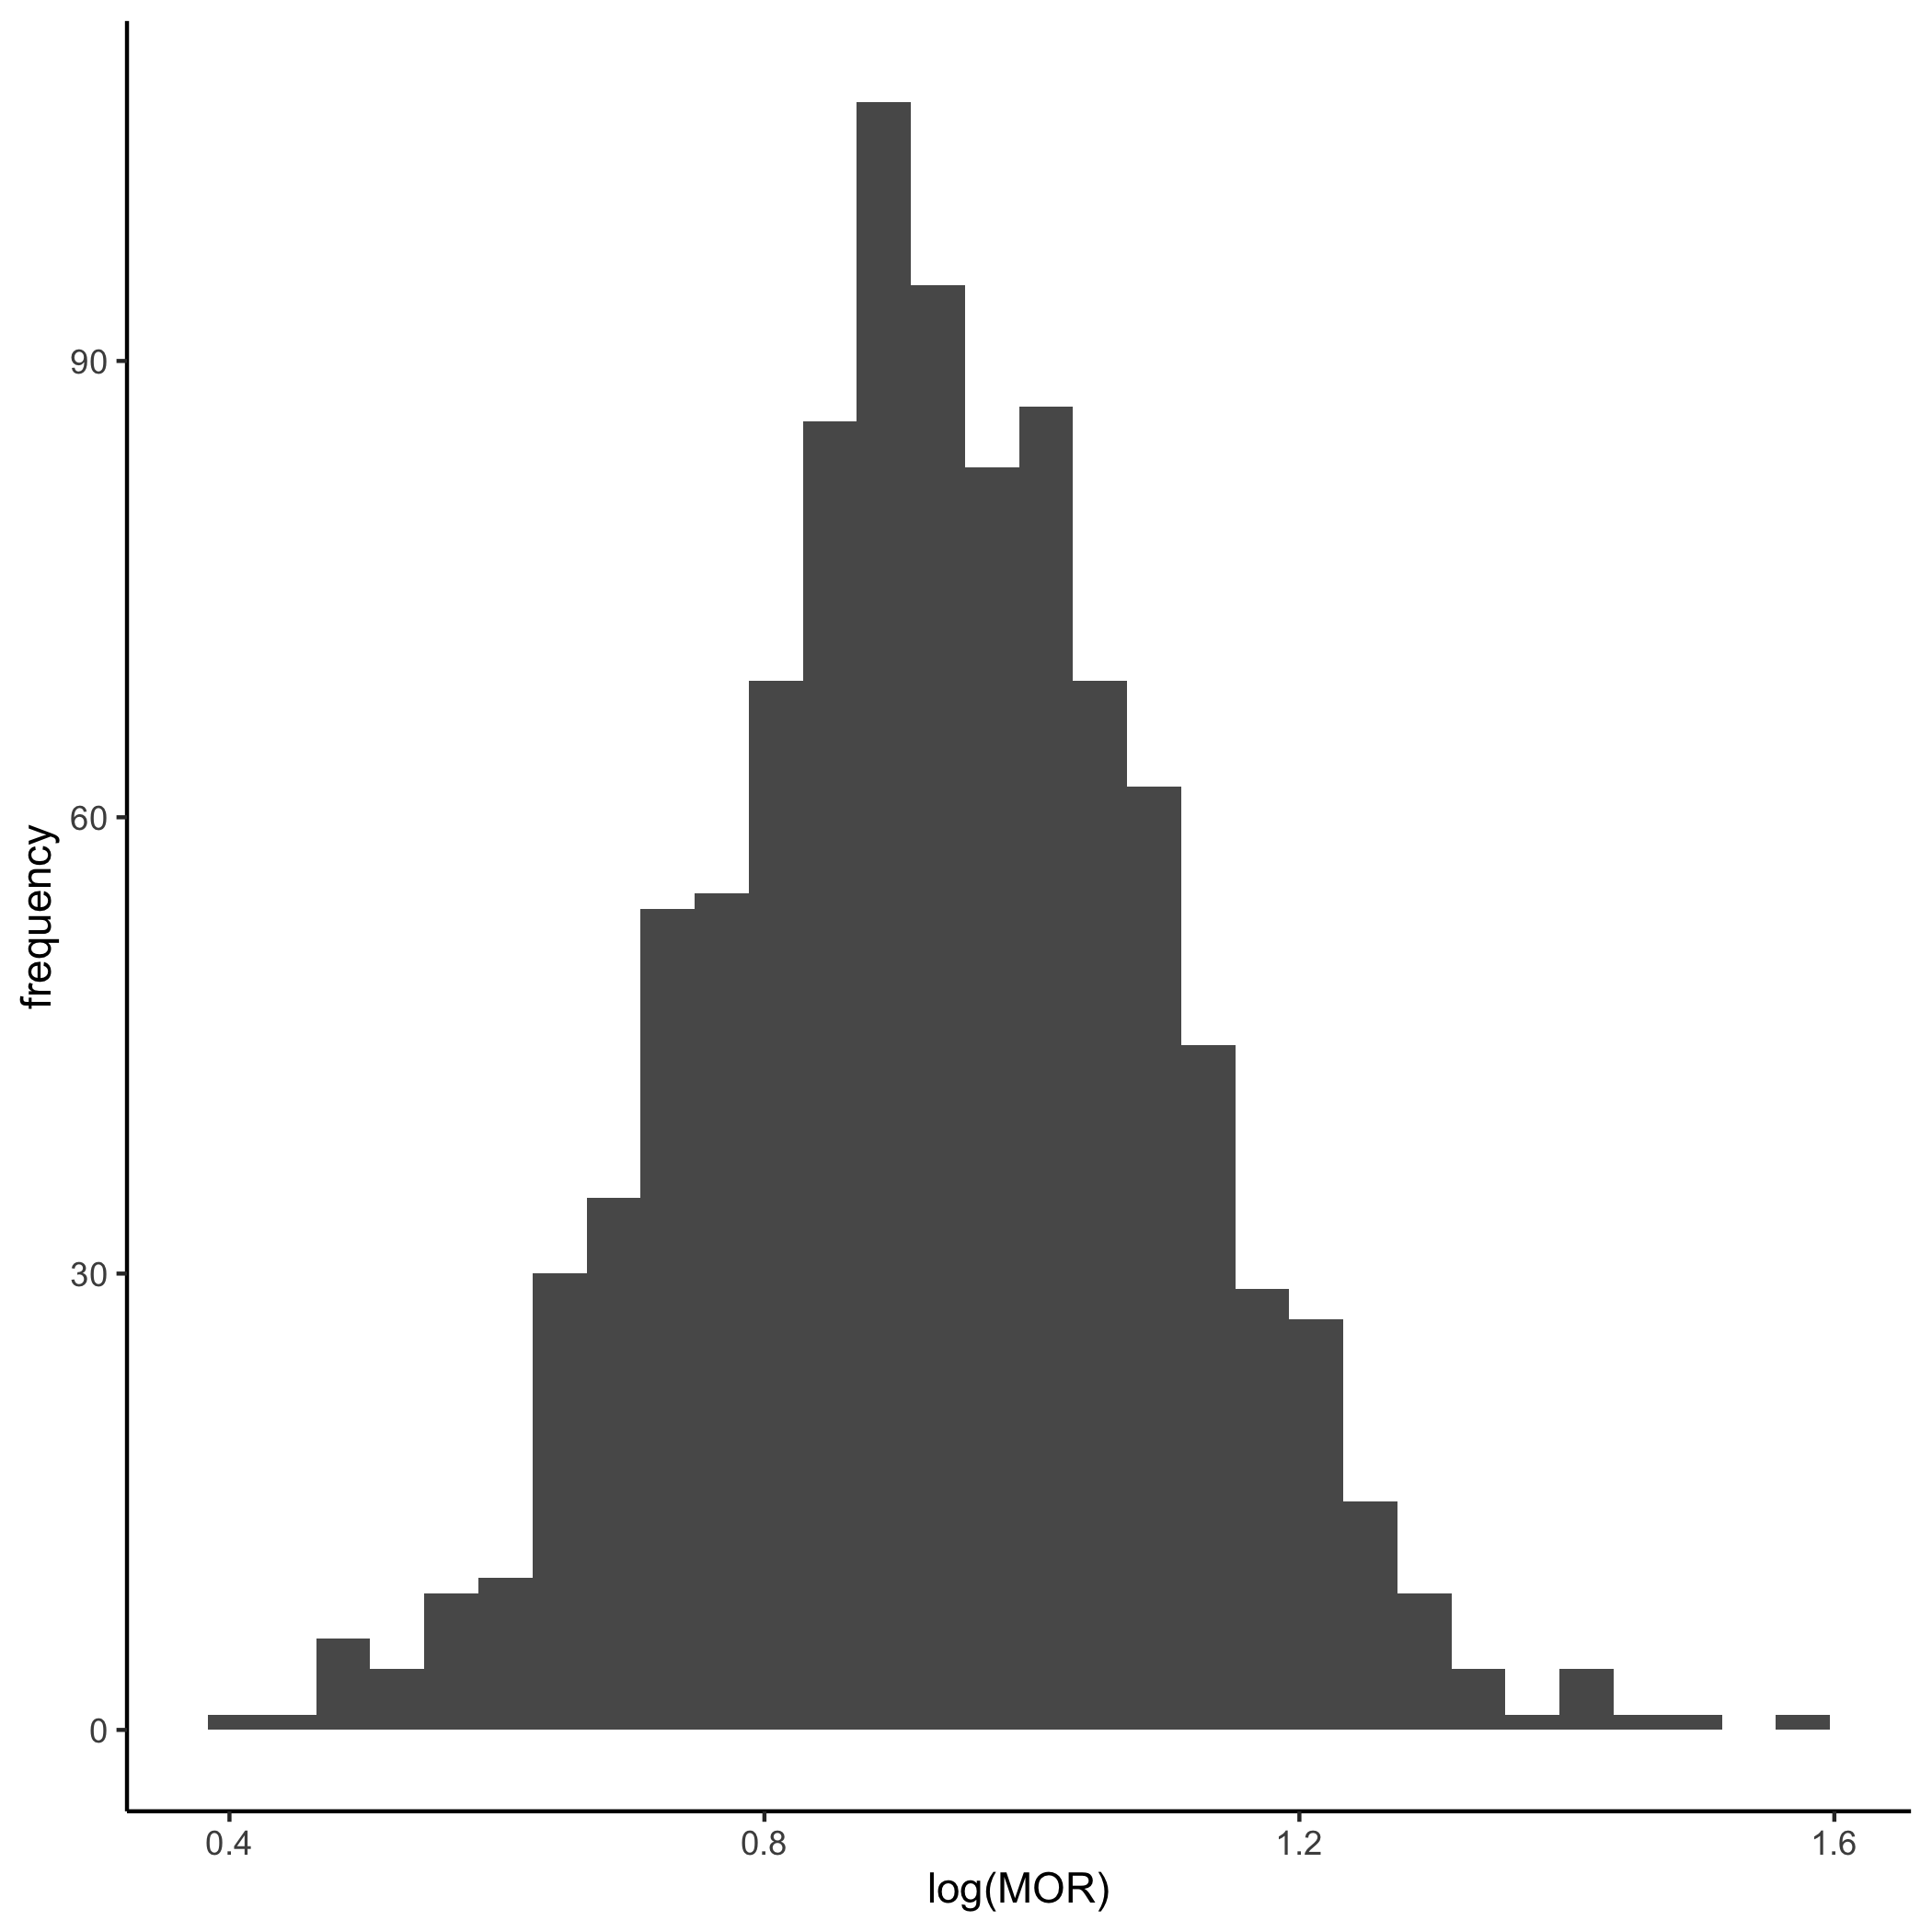
\includegraphics{../../plots/two-lvl-ran-slope/high-prev/hist_50_30_two_lvl_slp_high_prev.png}

}

\caption{For cluster size 30}

}

\end{minipage}%
%
\begin{minipage}[t]{0.50\linewidth}

{\centering 

\raisebox{-\height}{

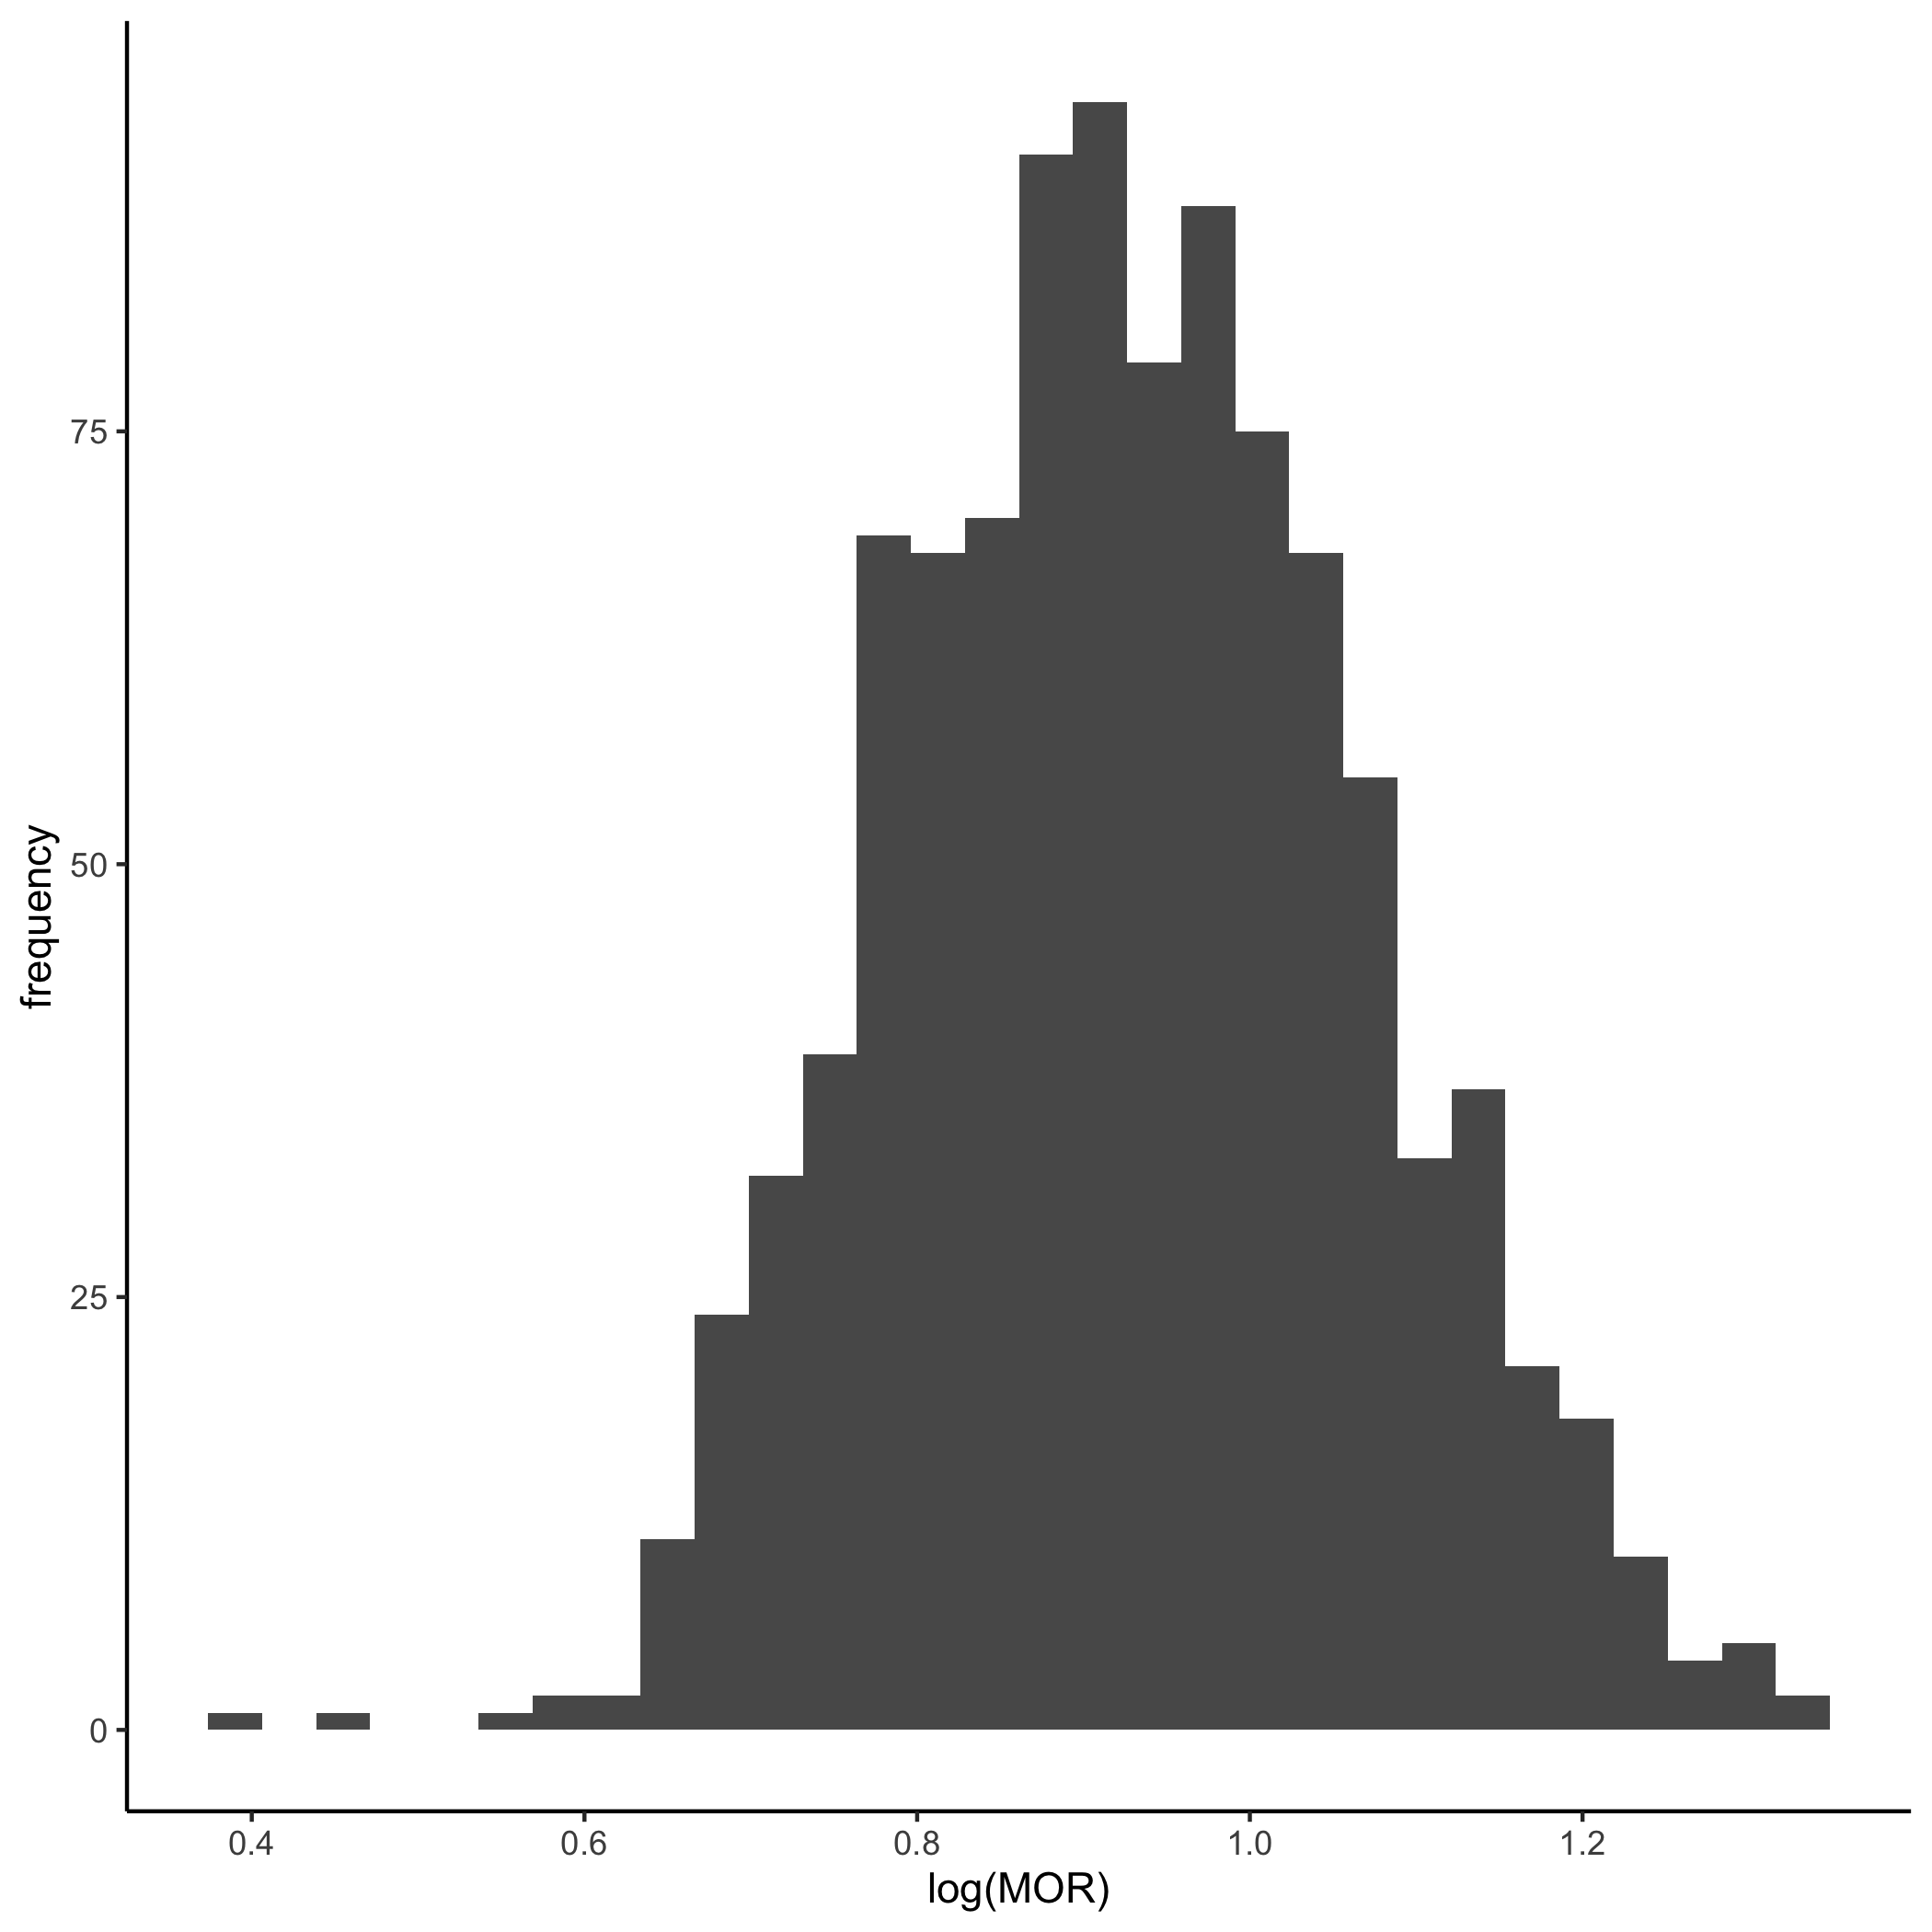
\includegraphics{../../plots/two-lvl-ran-slope/high-prev/hist_50_50_two_lvl_slp_high_prev.png}

}

\caption{For cluster size 50}

}

\end{minipage}%

\end{figure}

\newpage

\hypertarget{histograms-for-logwidehatmor-when-number-of-cluster-is-100}{%
\section{\texorpdfstring{Histograms for \(log(\widehat{MOR})\) When
Number of Cluster is
100}{Histograms for log(\textbackslash widehat\{MOR\}) When Number of Cluster is 100}}\label{histograms-for-logwidehatmor-when-number-of-cluster-is-100}}

\vspace{5mm}

\begin{figure}

\begin{minipage}[t]{0.50\linewidth}

{\centering 

\raisebox{-\height}{

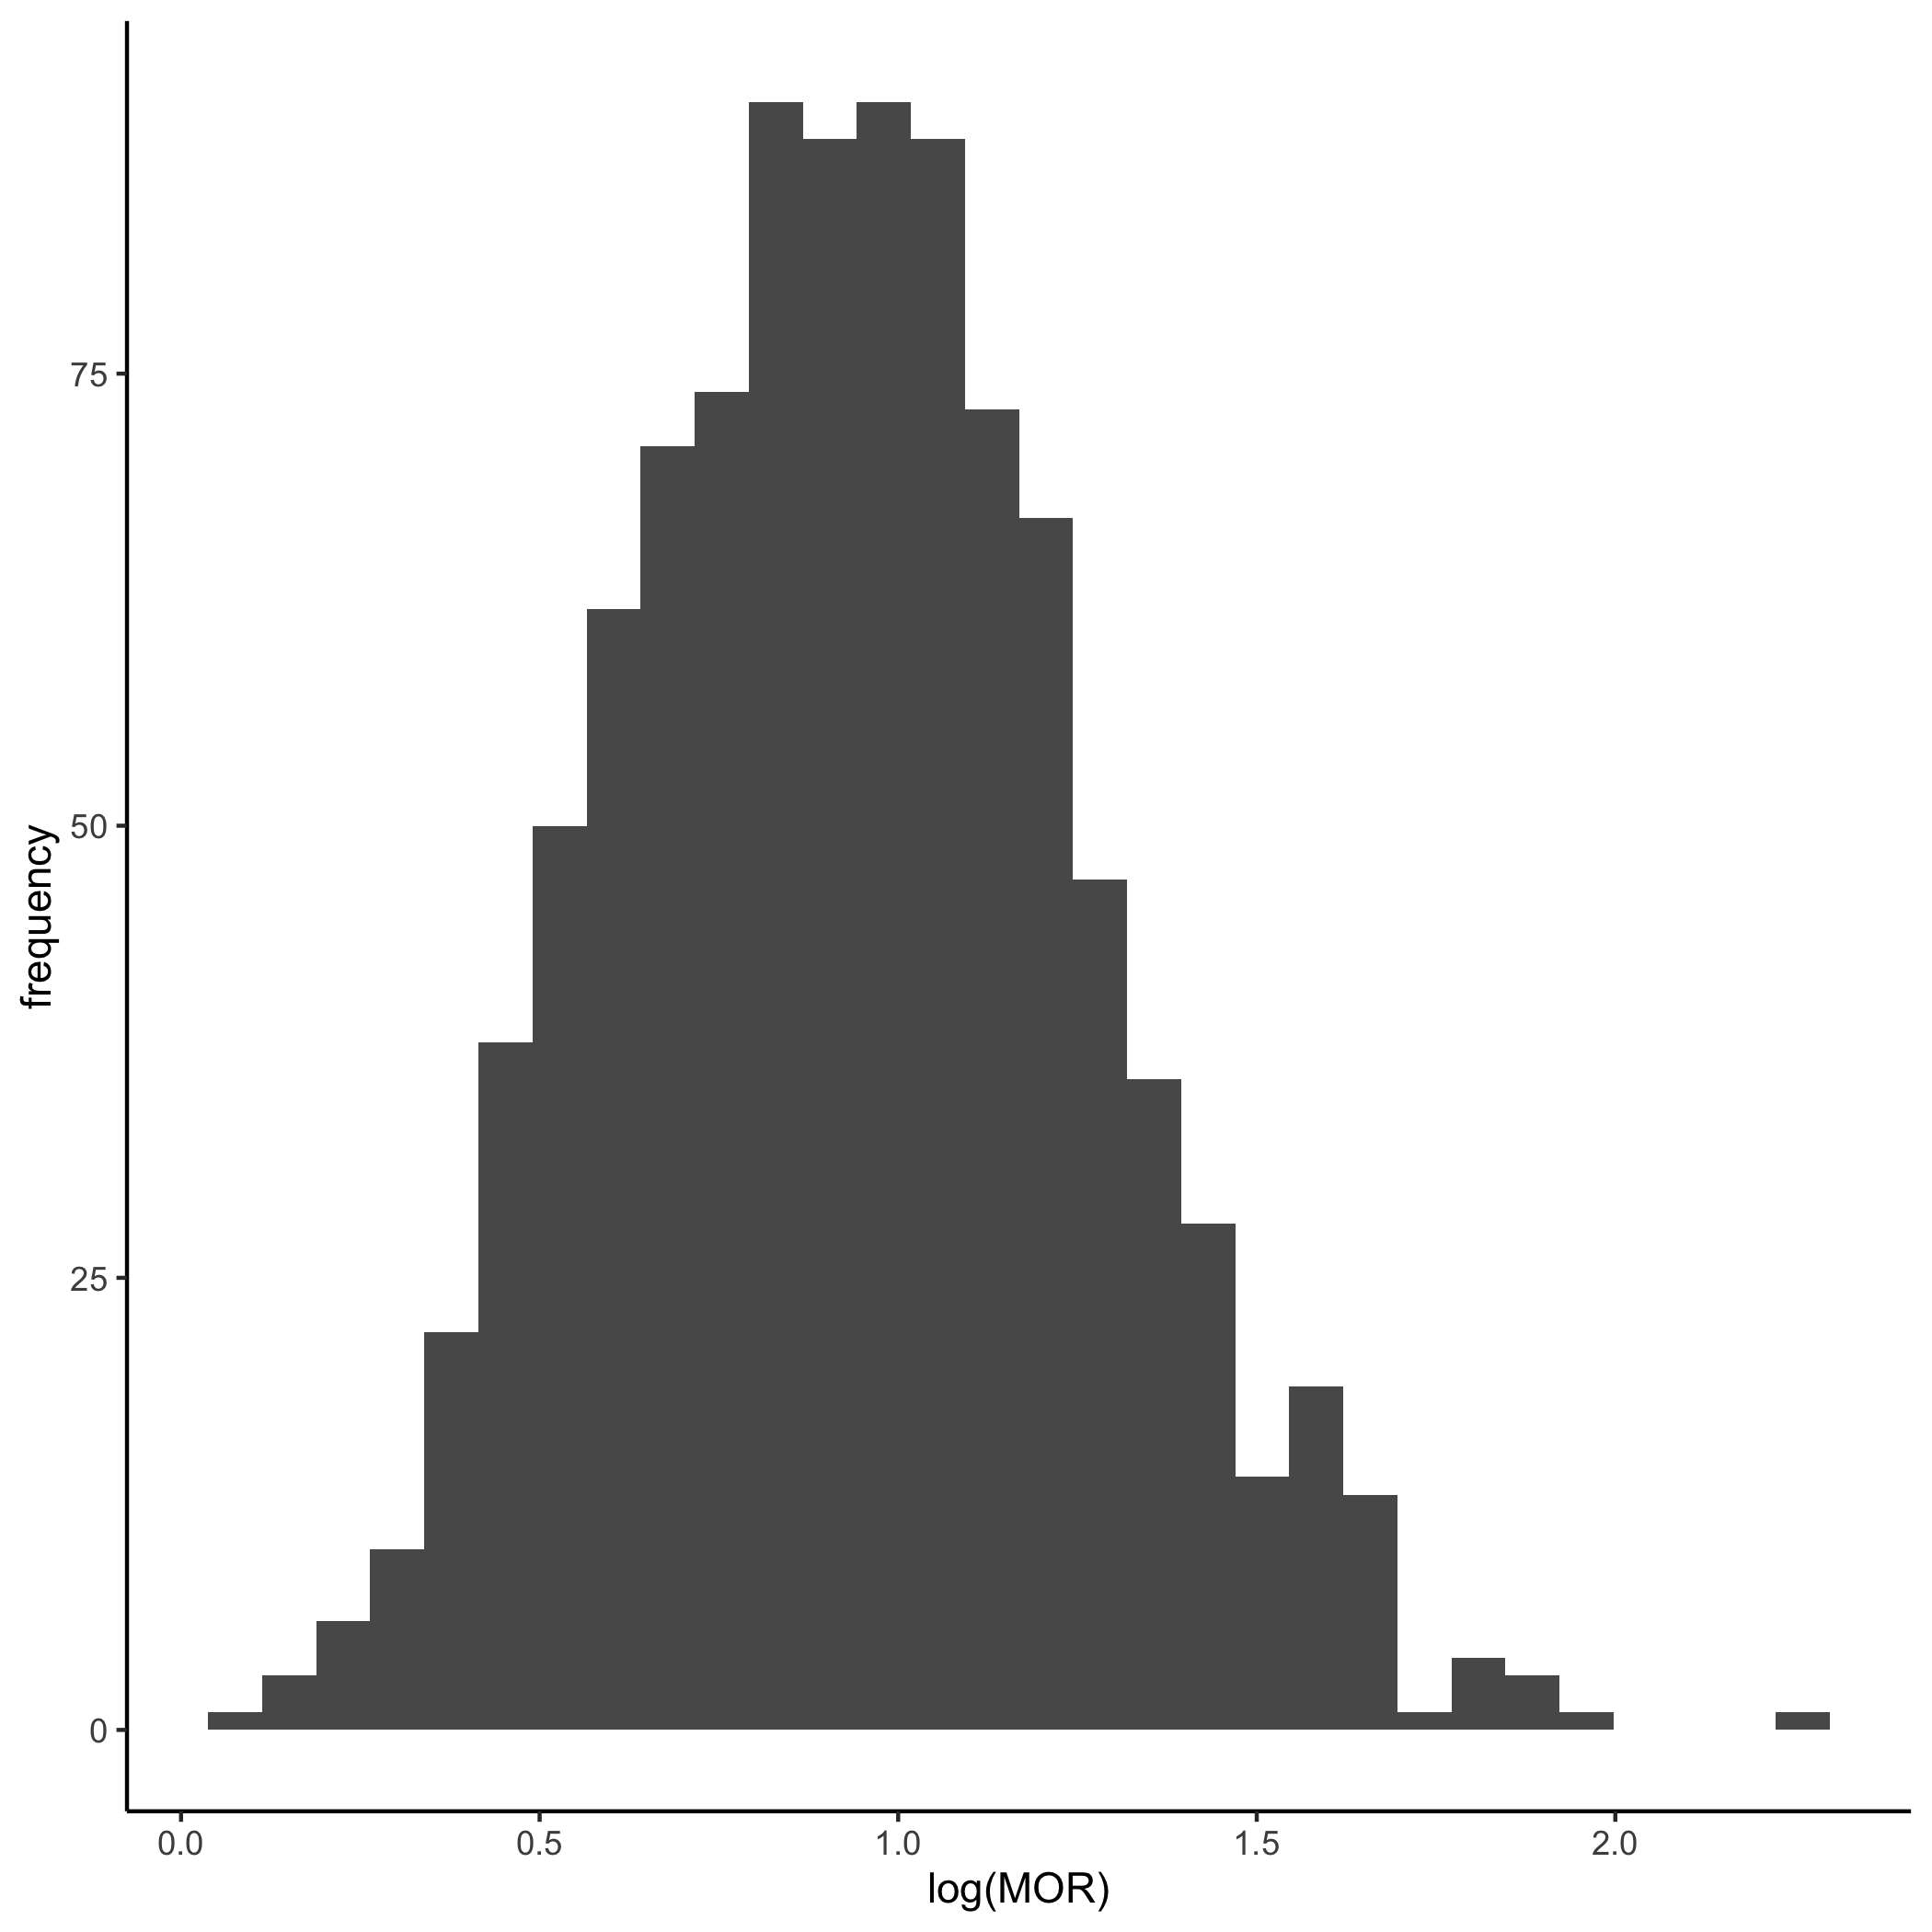
\includegraphics{../../plots/two-lvl-ran-slope/high-prev/hist_100_5_two_lvl_slp_high_prev.png}

}

\caption{For cluster size 5}

}

\end{minipage}%
%
\begin{minipage}[t]{0.50\linewidth}

{\centering 

\raisebox{-\height}{

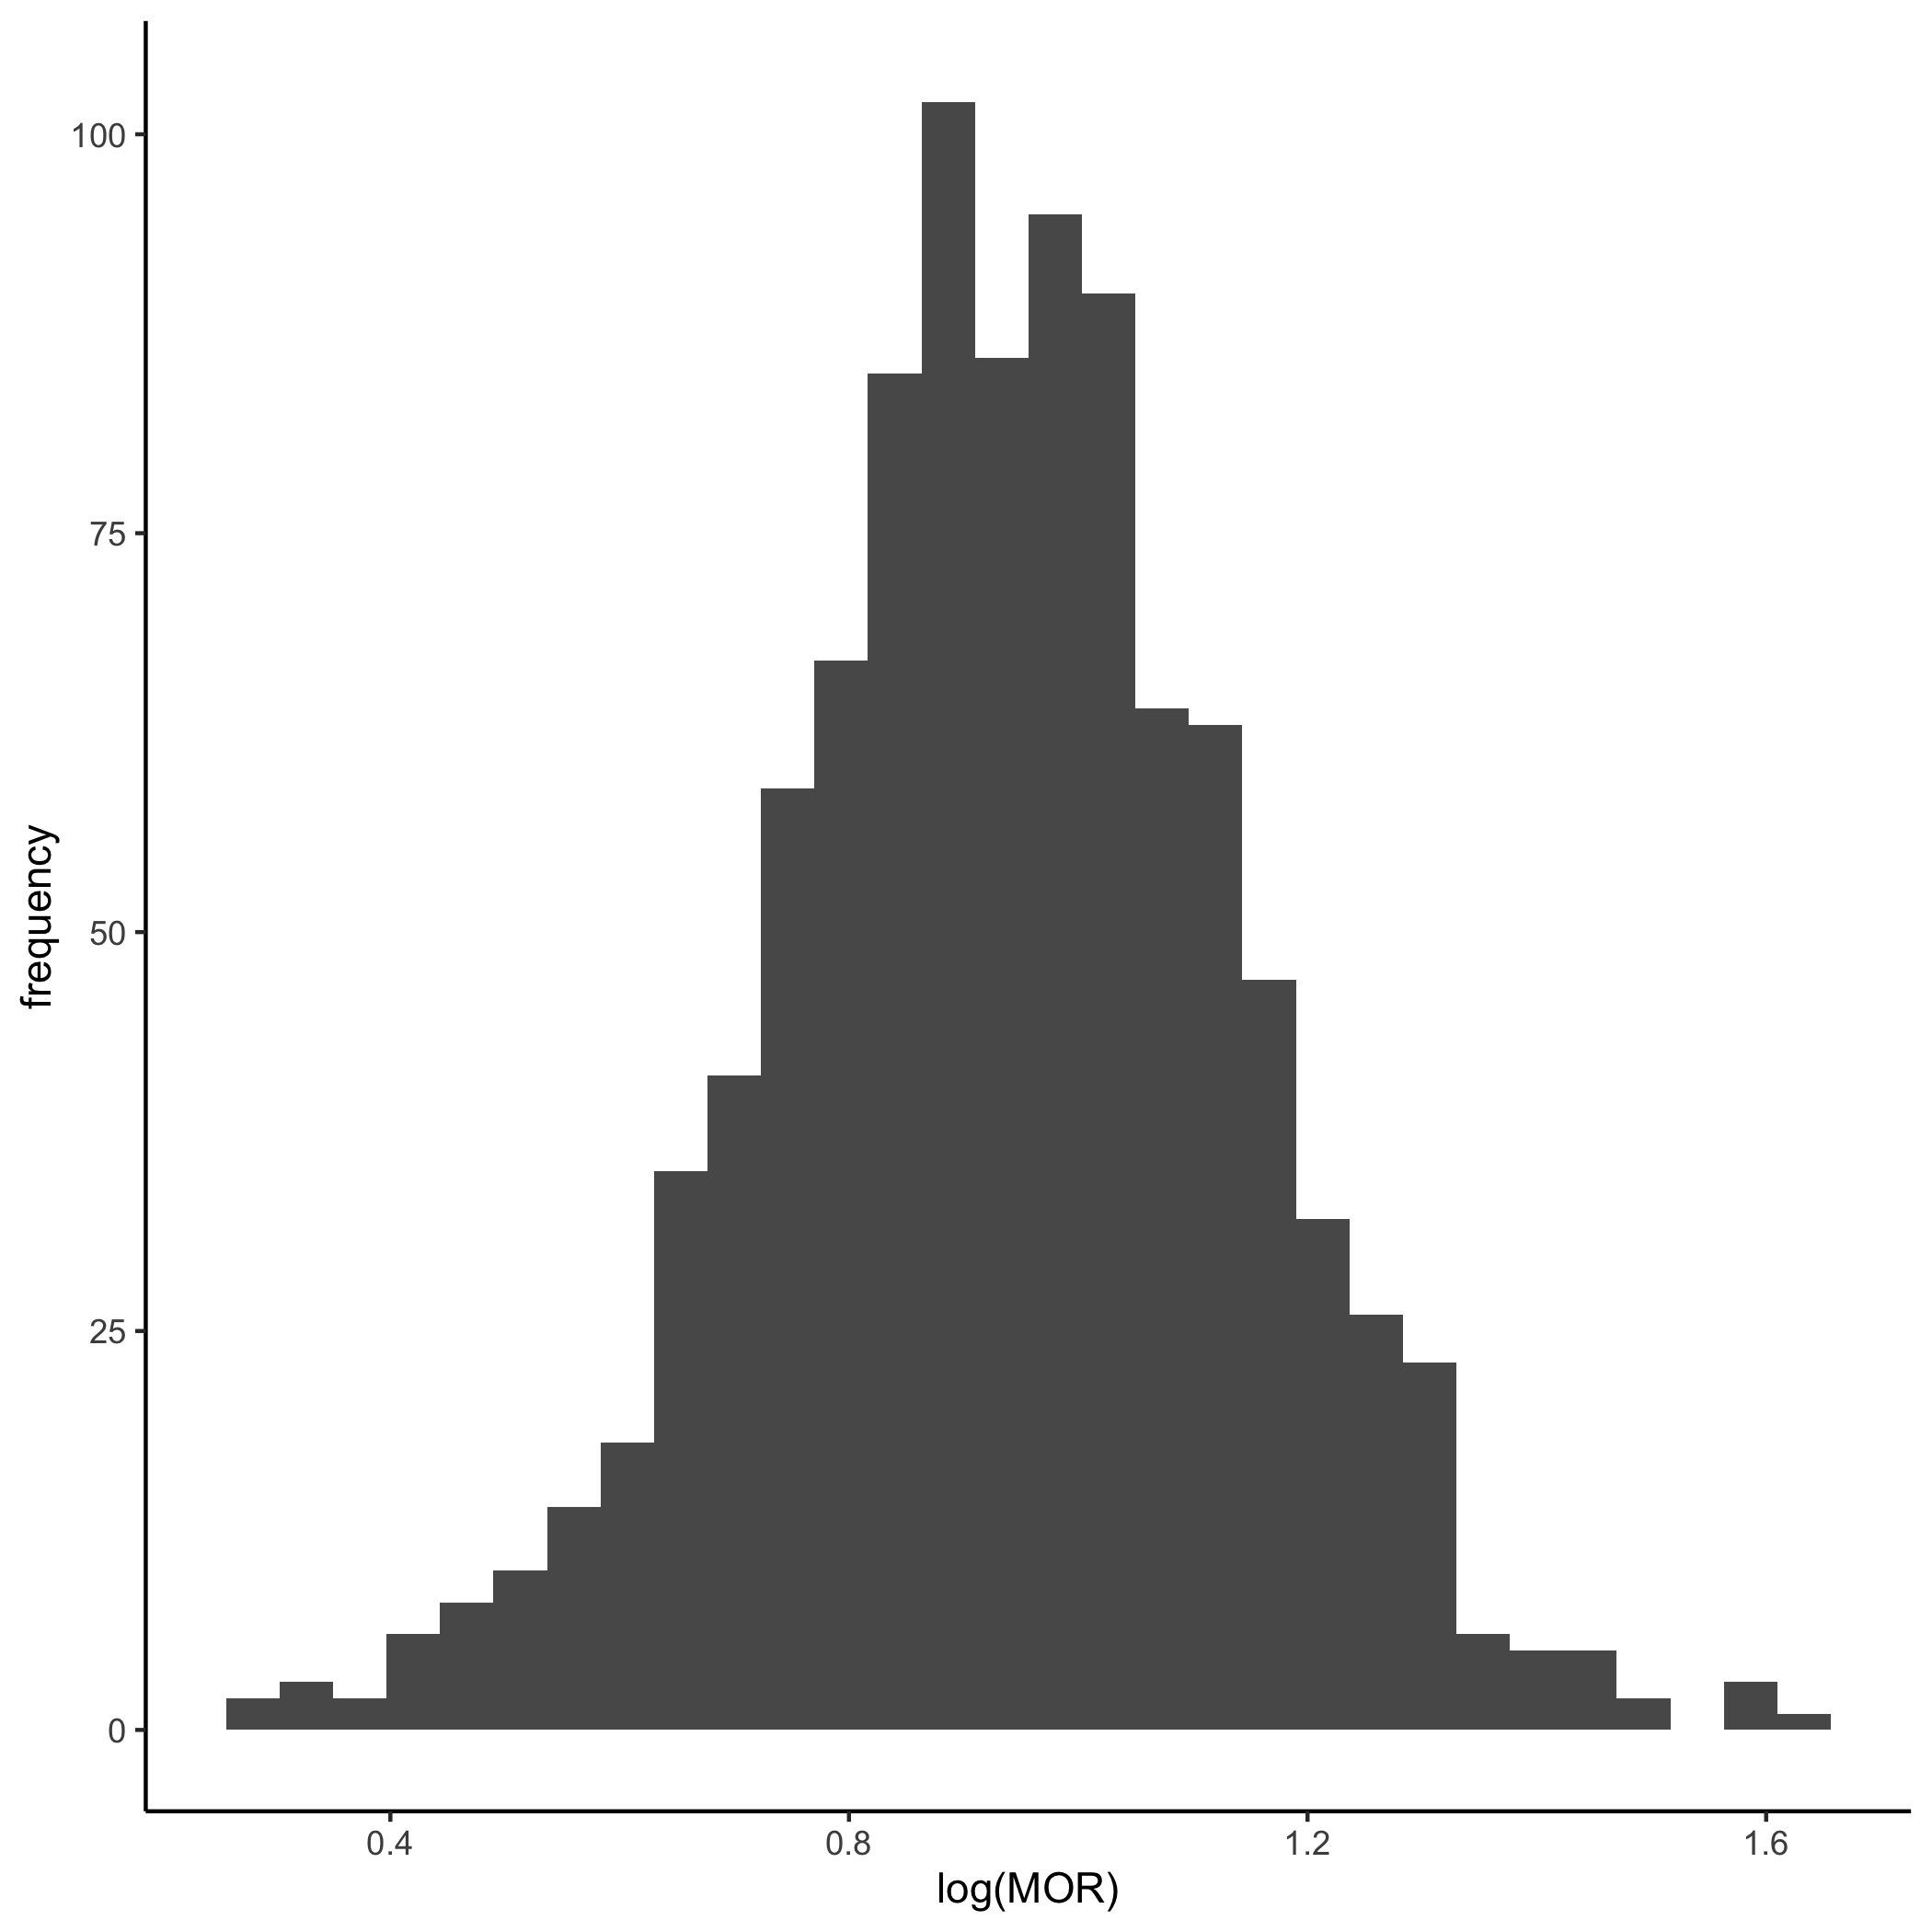
\includegraphics{../../plots/two-lvl-ran-slope/high-prev/hist_100_10_two_lvl_slp_high_prev.png}

}

\caption{For cluster size 10}

}

\end{minipage}%
\newline
\begin{minipage}[t]{\linewidth}

{\centering 

~

}

\end{minipage}%
\newline
\begin{minipage}[t]{0.50\linewidth}

{\centering 

\raisebox{-\height}{

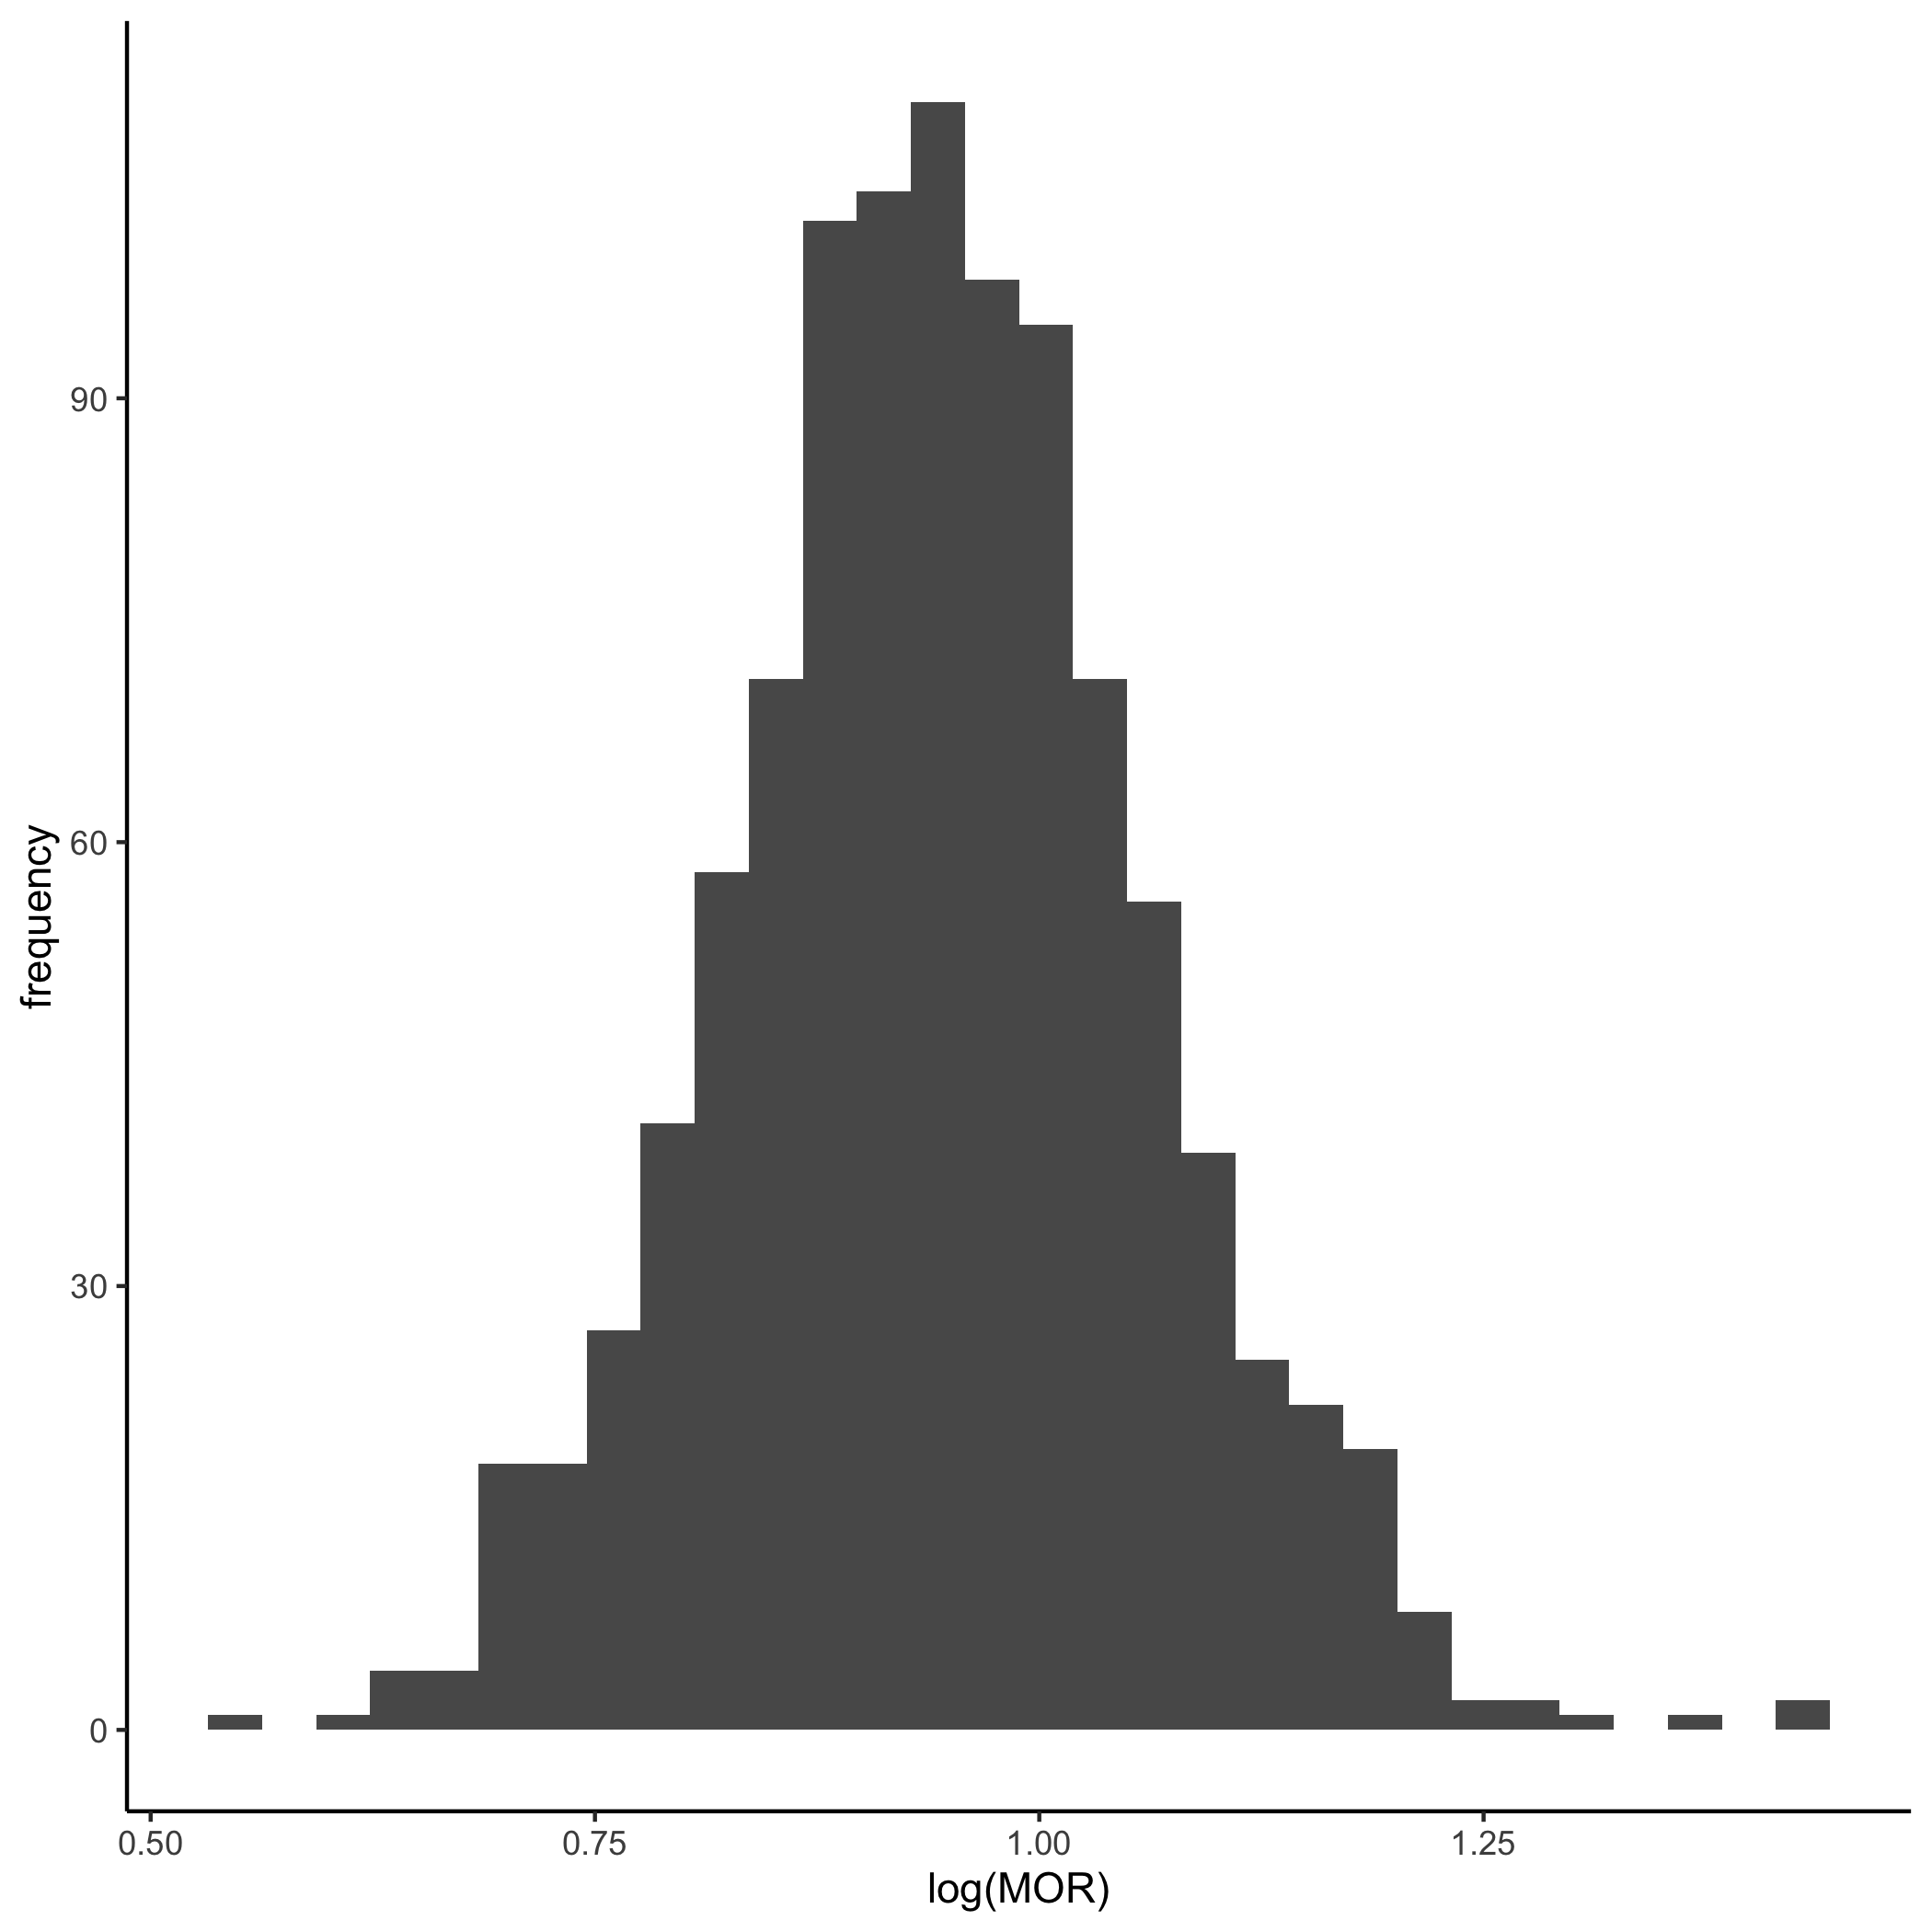
\includegraphics{../../plots/two-lvl-ran-slope/high-prev/hist_100_30_two_lvl_slp_high_prev.png}

}

\caption{For cluster size 30}

}

\end{minipage}%
%
\begin{minipage}[t]{0.50\linewidth}

{\centering 

\raisebox{-\height}{

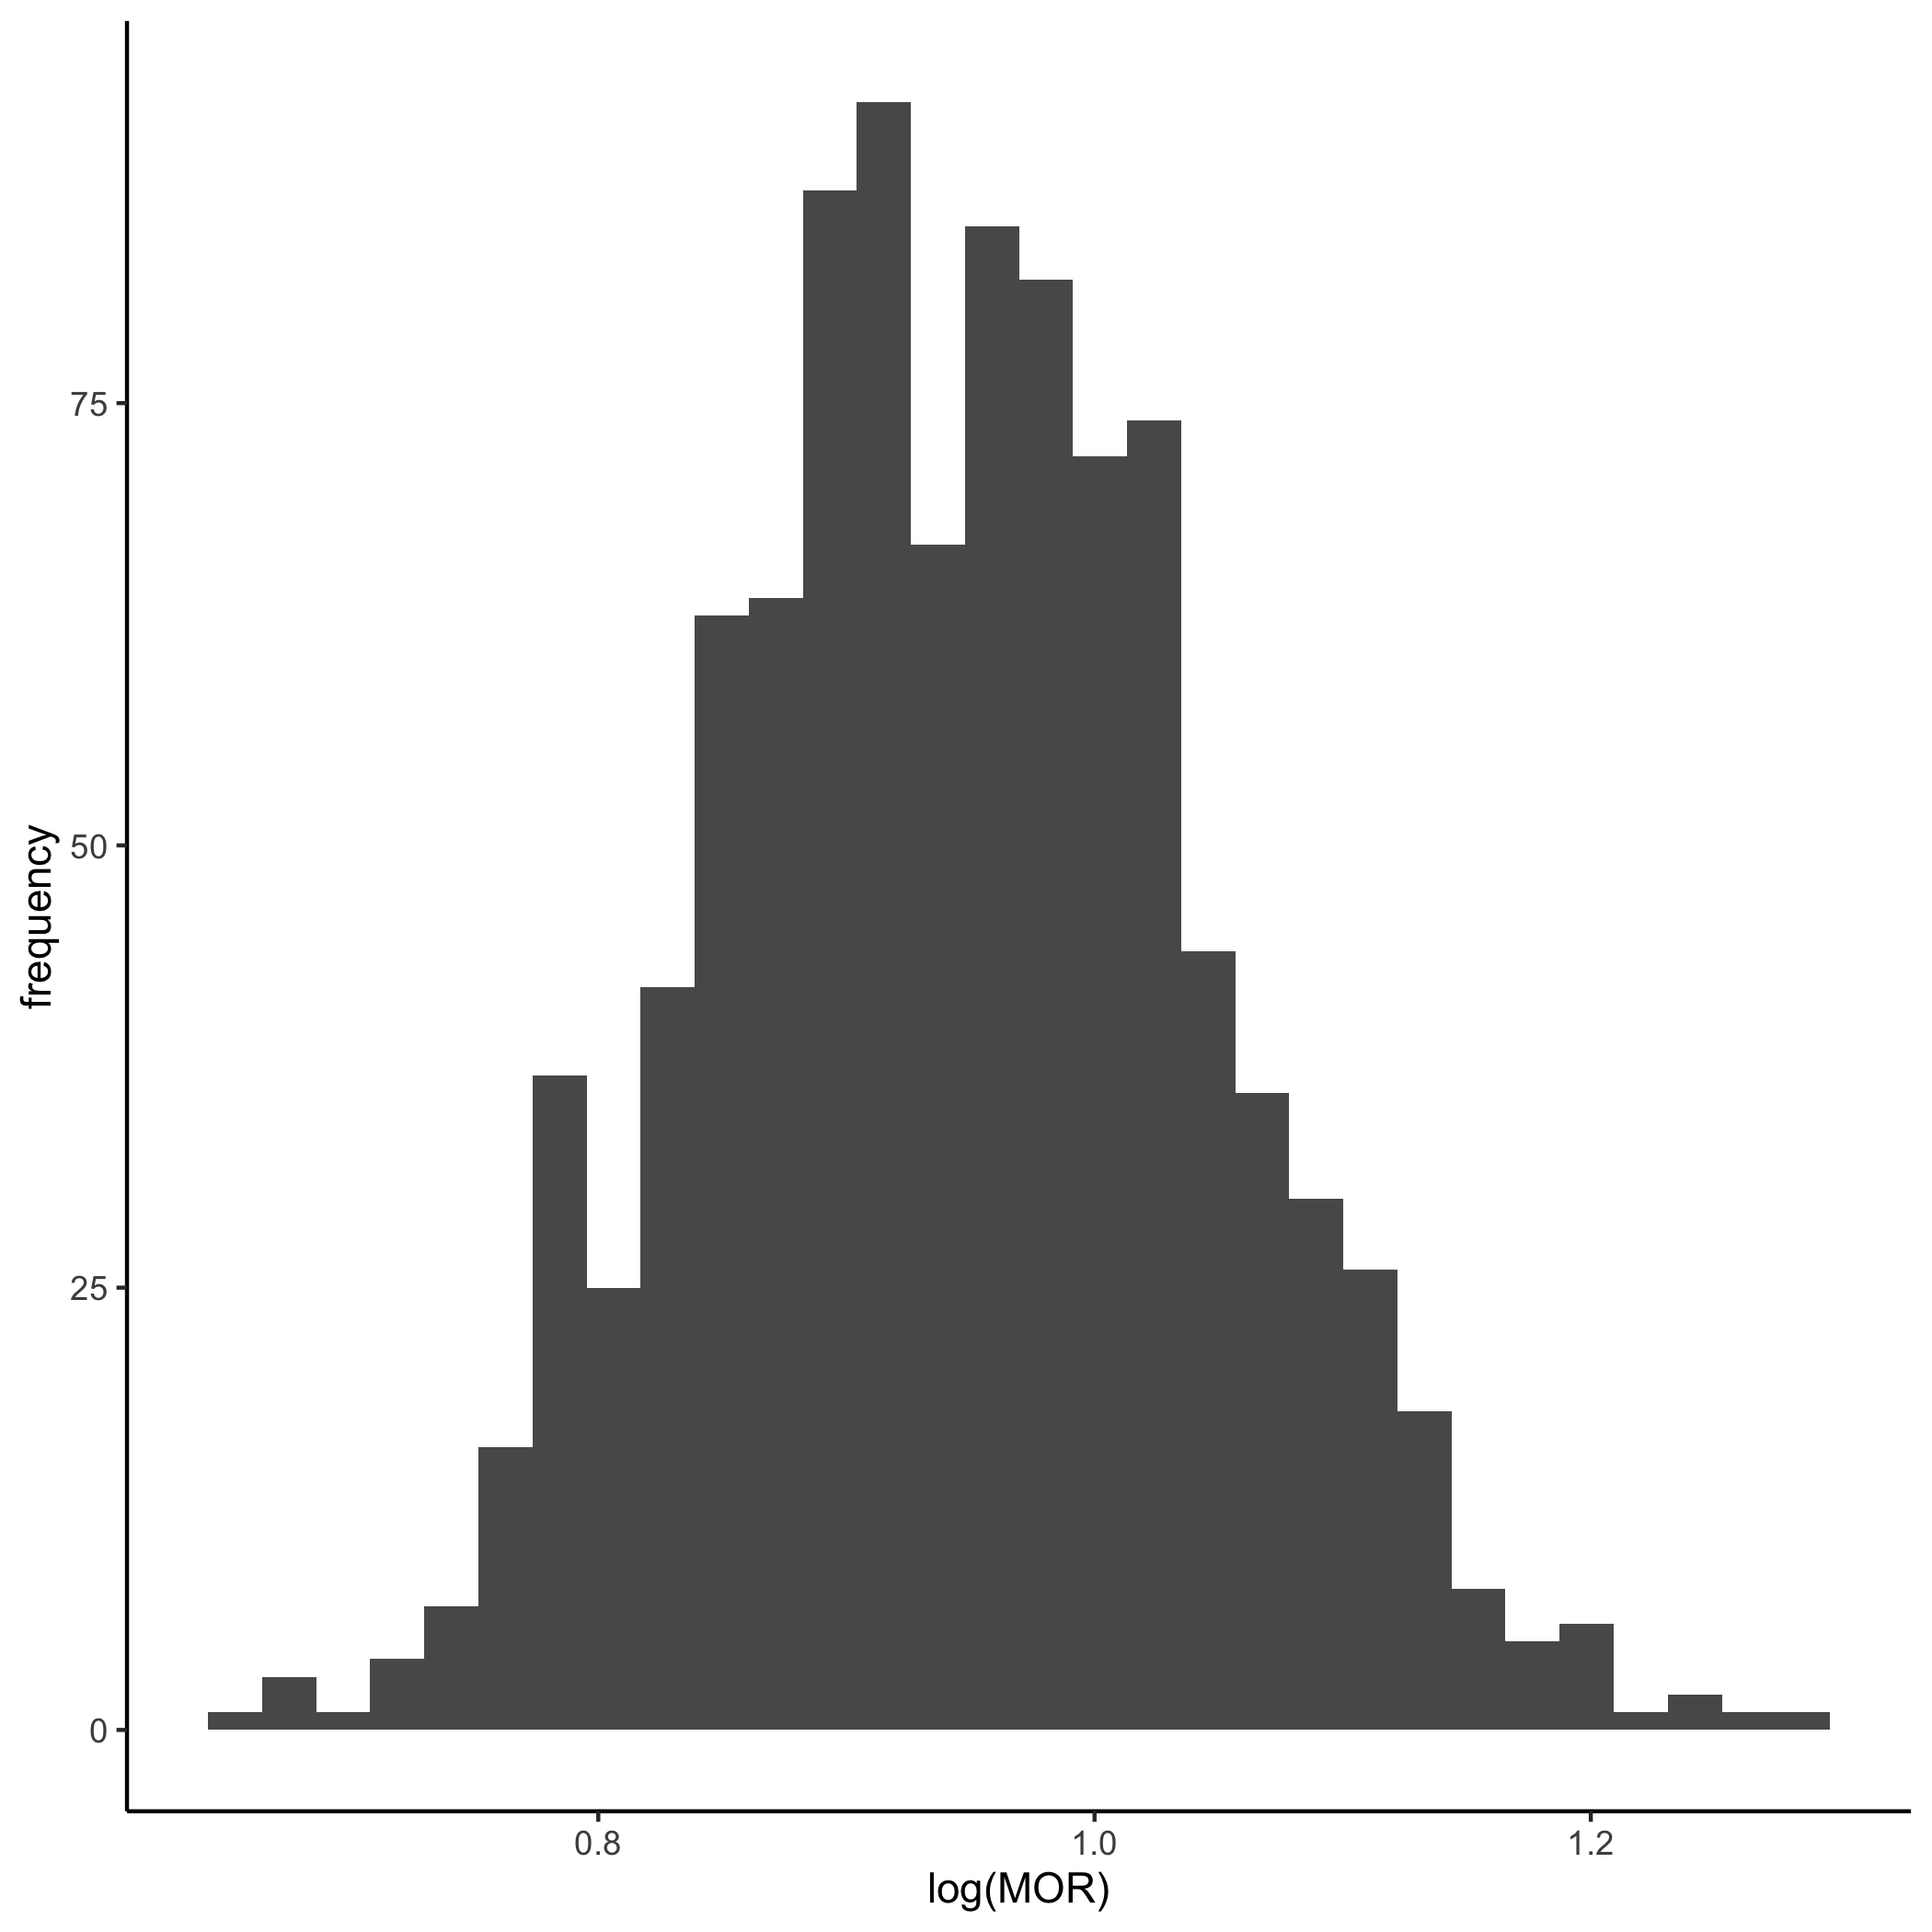
\includegraphics{../../plots/two-lvl-ran-slope/high-prev/hist_100_50_two_lvl_slp_high_prev.png}

}

\caption{For cluster size 50}

}

\end{minipage}%

\end{figure}

\newpage

\KOMAoptions{usegeometry,paper=landscape,pagesize}
\recalctypearea
\newgeometry{right=10mm,left=10mm}

\hypertarget{simulation-result-table}{%
\section{Simulation Result Table}\label{simulation-result-table}}

\begingroup

\fontsize{8pt}{12pt}\selectfont
\addtolength{\tabcolsep}{0.1pt}

\begin{threeparttable}
\begin{tabular}[t]{>{\centering\arraybackslash}m{1.1cm}>{\centering\arraybackslash}m{1.1cm}>{\centering\arraybackslash}m{1.1cm}>{\centering\arraybackslash}m{1.1cm}>{\centering\arraybackslash}m{1.1cm}>{\centering\arraybackslash}m{1.1cm}>{\centering\arraybackslash}m{1.1cm}>{\centering\arraybackslash}m{1.1cm}>{\centering\arraybackslash}m{1.1cm}>{\centering\arraybackslash}m{1.1cm}>{\centering\arraybackslash}m{1.1cm}>{\centering\arraybackslash}m{1.1cm}>{\centering\arraybackslash}m{1.1cm}>{\centering\arraybackslash}m{1.1cm}>{\centering\arraybackslash}m{1.1cm}>{\centering\arraybackslash}m{1.1cm}>{\centering\arraybackslash}m{1.1cm}}
\toprule
Number of Cluster & Cluster Size & $\widehat{\beta_0}$ & $\widehat{\beta_1}$ & $\widehat{\beta_2}$ & $\widehat{\sigma_{u_1}^2}$ & $\widehat{\sigma_{u_2}^2}$ & $\widehat{\sigma_{u_{12}}^2}$ & $MOR$ & $\widehat{MOR}$ & Relative Bias (\%) & $\widehat{SE}_{MOR}$ & Simulation $\widehat{SE}_{MOR}$ & Ratio\textsuperscript{1} & CI coverage (95\%) & Runs used & Runs Required\\
\midrule
10 & 5 & 2.28 & 2.16 & 0.86 & 1.83 & 3.47 & -0.04 & 2.64 & 4.07 & 54.06 & 4.14 & 2.08 & 1.99 & 0.99 & 1000 & 1436\\
10 & 10 & 2.17 & 1.98 & 0.85 & 1.38 & 2.94 & -0.10 & 2.62 & 3.20 & 22.10 & 2.25 & 1.81 & 1.25 & 0.98 & 1000 & 1038\\
10 & 30 & 2.02 & 1.78 & 0.72 & 0.98 & 1.97 & -0.03 & 2.60 & 2.58 & -0.93 & 1.49 & 1.46 & 1.02 & 0.93 & 1000 & 1001\\
10 & 50 & 2.02 & 1.76 & 0.69 & 0.95 & 1.91 & -0.06 & 2.60 & 2.53 & -2.77 & 1.39 & 1.40 & 0.99 & 0.90 & 1000 & 1000\\
\midrule
30 & 5 & 2.16 & 1.89 & 0.76 & 1.50 & 2.82 & -0.05 & 2.61 & 3.43 & 31.35 & 1.95 & 1.80 & 1.08 & 0.98 & 1000 & 1009\\
30 & 10 & 2.04 & 1.79 & 0.72 & 1.03 & 2.13 & 0.00 & 2.60 & 2.64 & 1.41 & 1.47 & 1.46 & 1.00 & 0.95 & 1000 & 1000\\
30 & 30 & 1.99 & 1.75 & 0.70 & 0.97 & 1.96 & -0.03 & 2.60 & 2.56 & -1.45 & 1.24 & 1.24 & 1.00 & 0.94 & 1000 & 1000\\
30 & 50 & 2.01 & 1.75 & 0.68 & 1.00 & 1.97 & -0.01 & 2.60 & 2.59 & -0.33 & 1.20 & 1.21 & 0.99 & 0.92 & 1000 & 1000\\
\midrule
50 & 5 & 2.06 & 1.81 & 0.71 & 1.20 & 2.41 & -0.05 & 2.61 & 2.88 & 10.39 & 1.63 & 1.55 & 1.05 & 0.98 & 1000 & 1000\\
50 & 10 & 2.01 & 1.77 & 0.69 & 1.01 & 2.12 & 0.01 & 2.60 & 2.60 & 0.07 & 1.34 & 1.35 & 0.99 & 0.96 & 1000 & 1000\\
50 & 30 & 2.00 & 1.74 & 0.67 & 0.98 & 1.98 & -0.03 & 2.60 & 2.57 & -1.14 & 1.18 & 1.19 & 0.99 & 0.93 & 1000 & 1000\\
50 & 50 & 2.00 & 1.74 & 0.69 & 0.97 & 1.95 & -0.02 & 2.60 & 2.56 & -1.47 & 1.15 & 1.15 & 1.00 & 0.93 & 1000 & 1000\\
\midrule
100 & 5 & 2.03 & 1.77 & 0.69 & 1.08 & 2.12 & -0.02 & 2.60 & 2.70 & 3.78 & 1.40 & 1.38 & 1.01 & 0.98 & 1000 & 1000\\
100 & 10 & 1.99 & 1.73 & 0.68 & 1.01 & 1.97 & -0.03 & 2.60 & 2.60 & 0.21 & 1.22 & 1.23 & 0.99 & 0.96 & 1000 & 1000\\
100 & 30 & 2.00 & 1.75 & 0.67 & 1.00 & 1.97 & -0.01 & 2.60 & 2.59 & -0.24 & 1.12 & 1.13 & 1.00 & 0.94 & 1000 & 1000\\
100 & 50 & 1.99 & 1.74 & 0.68 & 0.99 & 1.98 & 0.00 & 2.60 & 2.59 & -0.30 & 1.10 & 1.10 & 1.00 & 0.94 & 1000 & 1000\\
\bottomrule
\end{tabular}
\begin{tablenotes}
\item \textit{Note: } 
\item The mean prevalence for this simulation is 79\%
\item[1] Ratio$\;=\;\dfrac{\widehat{SE}_{MOR}}{Simulation\;\widehat{SE}_{MOR}}$
\end{tablenotes}
\end{threeparttable}

\endgroup

\vspace{10mm}

\newpage

Here,

\begin{itemize}
\tightlist
\item
  True \(\sigma^2_{u_1}\) = \(1\), \(\sigma^2_{u_2}\) = \(2\),
  \(\sigma^2_{u_{12}}\) = \(0\)
\item
  True Values of \(\beta_0 = 2\), \(\beta_1 = 1.75\), \(\beta_2 = 0.67\)
\item
  ``Runs used'' column represent how many simulation runs were used to
  calculate the numbers in the corresponding row.
\end{itemize}



\end{document}
